\documentclass[a4paper,11pt]{article}
\usepackage{amsmath,amssymb,graphicx,hyperref}
\usepackage[left=2.7cm, right=2.7cm, top=2.7cm, bottom=2.7cm]{geometry}

\usepackage{tocloft} % For custom table of contents
\usepackage{xcolor}  % For link and text color
\usepackage{hyperref} % For hyperlinks in TOC
\usepackage{minted}
\usepackage{subcaption}% multiple graphs side by side
\usepackage{booktabs} %these two makes tables look better
\usepackage{tabularx}
\usepackage{doi}
\usepackage{url}
\usepackage{cite}
\usepackage{epstopdf}


\definecolor{LightGray}{gray}{0.9}
% Set link colors
\hypersetup{
	colorlinks=true,
	linktoc=page,      % Makes only page numbers clickable
	linkcolor=blue,    % Link color (e.g., for TOC)
	urlcolor=cyan,     % URL link color
	citecolor=magenta  % Citation link color
}


% Custom TOC style
\renewcommand{\cfttoctitlefont}{\normalfont\large\bfseries} % TOC title
\renewcommand{\cftsecfont}{\bfseries}  % Bold section names
\renewcommand{\cftsecpagefont}{\color{blue}} % Page numbers blue
\renewcommand{\cftsecleader}{\cftdotfill{\cftdotsep}} % Dot leader
%\newcommand{\blackrule}{\noindent\rule{\textwidth}{0.5pt}}

% Increase spacing in TOC
\setlength{\cftbeforesecskip}{5pt} % Space before section entries
\setlength{\cftbeforesubsecskip}{2pt} % Space before subsection entries



\title{\textbf{The Higgs boson search at the Large Hadron Collider}}

\author{
	Edwin Varghese\\[10pt]
	\small Department of Physics, Royal Holloway, University of London, Egham Hill, TW20 0EX, U.K.\\
	\texttt{\small zkap069@live.rhul.ac.uk}
}

\date{}

\begin{document}
	
	\maketitle
	
	\begin{abstract}
		This review summarises the phenomenology and experimental searches for the Higgs boson conducted at the Large Hadron Collider. It includes descriptions of Higgs boson production, decay modes and a focused discussion of the channels relevant for discovery and the vector boson fusion channel. The production modes --- gluon-gluon fusion, vector boson fusion, associated production with weak gauge bosons, and heavy quark associated production --- are discussed in detail alongside next-to-leading and higher-order QCD and electroweak corrections. The analysis further explores the principal decay channels --- including fermionic, vector boson, and loop-induced processes --- with particular focus on the clean signatures provided by the $ H \rightarrow \gamma \gamma$ and $H \rightarrow ZZ \rightarrow 4 \ell$ channels, namely the discovery channels. The role of vector boson fusion in enhancing discovery sensitivity across intermediate to high Higgs mass ranges is also highlighted. Results from TeVatron and LEP are briefly mentioned to illustrate the experimental evolution leading to the discovery of the Higgs boson at the LHC, and to outline the statistical methodologies employed in signal extraction.
		
		
	\end{abstract}
	
	
	\newpage
	\tableofcontents
	\vspace{-5pt}
	\newpage

	
	\section{Introduction} 

Hadron colliders have played an important role in addressing fundamental questions of particle physics, and will remain our primary source for testing the Standard Model (SM). The electroweak theory, described by the gauge symmetry group $SU(2)_L \times U(1)_Y$, was developed in the 1960s to unify the weak and electromagnetic interactions of quarks and leptons. In conjunction with later developments in quantum chromodynamics, the theory of the strong interactions between the coloured quarks described by $SU(3)_C$, yields the Standard Model gauge group: $SU(3)_C \times SU(2)_L \times U(1)_Y$. This model provides a framework that describes the strong, weak and electromagnetic interactions, is perturbative at sufficiently high energies and renormalisable, thus describes these interactions at the quantum level \cite{Djouadi:2005gi}.\\ 

Initially, the mechanism responsible for electroweak symmetry breaking was still unknown. As it stood, the electroweak theory described massless weak gauge bosons and long range weak interactions. A massive carrier produces a Yukawa potential, $V_{\text{Yukawa}}(r) \propto e^ {-\alpha m r}/r$, which is exponentially suppressed. If the weak bosons were massless, there would be no exponential suppression; weak forces would act over long distances and would produce additional forces between atoms, nuclei and bulk bodies that would have been detected. However, simply inserting explicit mass terms by hand would violate gauge invariance and make the theory non-renormalisable \cite{THOOFT1972189}. The electroweak symmetry had to be spontaneously broken, and this was realised via the Higgs mechanism. This is a process in which the $SU(2)$ doublet of complex scalar fields acquires a non-zero vacuum expectation value; three of the four degrees of freedom of the doublet are absorbed by the $W^\pm$ and $Z$ bosons which gives the weak vector bosons mass and a longitudinal polarisation\cite{Higgs:1964pj}. Through this mechanism, the weak vector bosons acquired mass in a way, as was shown by a proof from 't Hooft and Veltman \cite{tHooft:1972ikm},  that respects the requirements of renormalisability and unitarity \cite{tHooft:1971qjg}. The remaining degree of freedom corresponds to a single neutral scalar particle --- the Higgs boson \cite{Englert:1964et}. The fermion masses are generated through a Yukawa interaction with the same scalar field and its conjugate field \cite{Djouadi:2005gi}.\\

Measurements taken by experiments --- such as LEP, SLC, and TeVatron --- show that the Standard Model provides the correct effective description of the strong and electroweak interactions at the energies probed by those experiments. The couplings of quarks and leptons to the electroweak gauge bosons have been determined with high precision and agree with the model’s predictions \cite{Djouadi:2005gi}; likewise, measurements of trilinear gauge boson couplings, done by the DELPHI experiment, saw no evidence for deviations from the Standard Model  predictions in any of their results \cite{DELPHI:2001kqh}. The $SU(3)_C$ gauge description of the strong interaction has also been extensively tested. Yet, the scalar sector of the Standard Model was not explored and the Higgs particle was yet to be observed; high-precision electroweak  data yield only indirect constraints on its mass via their sensitivity to loop corrections \cite{Buescher:2005re}. Following the discovery of the W$^{\pm}$ bosons \cite{UA1:1983mne} and Z boson \cite{UA2:1983mlz} at CERN in 1983, investigating the mechanism of electroweak symmetry breaking became a central focus of particle physics. Determining the Higgs boson mass, the Higgs width, its quantum numbers, and  measuring  Higgs couplings to itself, gauge bosons, fermions, would be a decisive test for the Standard Model. Therefore, this was a major goal for the next generation of high-energy collider experiments.
	
	\section{Higgs production and decay in the Standard Model}
	
	\subsection{Higgs Boson Production} 
	The search for the Higgs boson has evolved through generations of high-energy particle colliders. The Large Electron-Positron Collider (LEP) established lower mass bounds and probed associated production channels; the Tevatron extended the sensitivity to higher mass ranges through proton-anti-proton collisions; and the Large Hadron Collider (LHC) ultimately enabled the discovery and precision measurement of the Higgs boson.\\
	
Commissioned in July 1989, LEP was a collider consisting of counter-rotating beams of electrons and positrons;  the LEP was initially run at 91.2 GeV, to study the W and Z bosons, and eventually reached a centre-of-mass energy of 209 GeV. Efforts were put in place to search for the Higgs Boson in their data; at the LEP energy scale, the dominant Higgs production mechanism is known as Higgs-strahlung\footnote{German for Higgs-radiation} ($e^+e^- \rightarrow ZH$) in which the electron-positron collision produces a virtual Z Boson and a Higgs particle. WW and ZZ fusion contributed at smaller rates. LEP searched for a light Higgs Boson; the centre-of-mass energies in the 189 to 109 GeV range provided sensitivity to the SM Higgs up to a mass of $m_H \sim 115$ GeV\cite{Raspereza:2002ni}. The ALEPH detector saw excess $\sim$ 115 GeV that was estimated to be a 3$\sigma$ deviation from the background. The combined results from DELPHI, OPAL, ALEPH and L3 saw excess 115 GeV that had 2.9 $\sigma$ deviation from background which was not enough to cross the conventionally required 5$\sigma$ discovery threshold \cite{Mori:2001qow}. The observed excess of events, seen mostly in the ALEPH data and in the four-jet channel (seen in Table \ref{tab:HiggsCandidates}), is compatible with a light Higgs Boson; the dominant decay at $\sim 114.4$ GeV is $H \rightarrow b\bar{b}$, producing two jets and two further jets are produced via the Z decay into two light quarks. Below this threshold, no statistically significant signal was found, thus excluding all Higgs masses below 114.4 GeV at 95\% CL \cite{Raspereza:2002ni}. Despite not achieving a direct Higgs discovery, LEP set the energy scale by establishing a lower bound on $m_H$ that the TeVatron and Large Hadron Collider would probe.\\

It is important to note that the LHC is a proton-proton collider, whereas TeVatron is a proton-anti-proton collider; the Higgs-strahlung production mechanism requires a quark-anti-quark initial state, thus, was suppressed at the LHC as the initial anti-quark must originate from the sea. On the other hand, the initial quarks and anti-quarks are valence, therefore both the CDF and D$\phi$ detectors concentrated their low-mass Higgs searches in the Higgs-strahlung production channels. The LHC and TeVatron also operate at different centre-of-mass energies; at $\sqrt{s} = 1.96$ TeV , TeVatron's Higgs cross-section is only 1.2pb whereas the LHC at $\sqrt{s} = 14$ TeV has a Higgs cross-section of 57.1 pb (refer to Table \ref{tab:HiggsCrossection}). One can deduce from Figure \ref{fig:TotalWidth at different TeVs}, the increase in centre-of-mass energy corresponds to a higher yield of Higgs Bosons. TeVatron was able to probe the light SM Higgs scale; the main decay mode at this scale is $H \rightarrow b\bar{b}$, where the $b$-quarks hadronise into jets. Both the gluon-fusion and vector boson fusion (VBF) channels produce jets that increase the background; by contrast, $qq \rightarrow ZH, WH$ channels produce W and Z bosons that decay into leptonic (electron and muon) jets which sophisticated algorithms at TeVatron can pick out with high purity \cite{D0:2013xld}. Requiring both clean leptonic jets and b-jets in conjunction with b-tagging techniques, background jets can be suppressed, leading to cleaner signatures.\\



\begin{table}[tb]
	\centering
	\caption{Based on table from \cite{Carena:2016hpv}. Production cross-sections (in pb) for a 125 GeV Higgs boson at centre-of-mass energies of TeVatron ($\sqrt{s} = 1.96$ TeV) and successive runs of the LHC ($\sqrt{s} = 7, 8, 13, 14$ TeV) .}
	\label{tab:HiggsCrossection}
	\begin{tabularx}{0.5\textwidth}{@{}l l@{}}
		\toprule
		\textbf{$\sqrt{s}$ (TeV)} & cross-section \textbf{(pb)}\\
		\midrule
		1.96  & 1.23 \\
		7  & 17.5 \\
		8  & 22.3 \\
		13 & 50.6 \\
		14 & 57.1 \\
		\bottomrule
	\end{tabularx}
\end{table}


\begin{table}[tb]
	\centering
	\caption{Based on table from \cite{Mori:2001qow}. Properties of the ten most significant Higgs boson candidate events observed at LEP, for $m_H = 115$ GeV. $E_{CM}$ is the centre-of-mass energy, $M_{rec}$ is the reconstructed mass. Excess is mainly in the ALEPH detector and involve four-jet final states.}
	\label{tab:HiggsCandidates}
	\begin{tabularx}{\textwidth}{@{}l l l l l@{}}
		\toprule
		\textbf{Detector} & \textbf{$E_{CM}$ (GeV)} & \textbf{Type} & \textbf{$M_{rec}$ (GeV)} & \textbf{Weighting} \\
		\midrule
		ALEPH  & 206.6 & 4-jet  & 114.1 & 1.76 \\
		ALEPH  & 206.6 & 4-jet  & 114.4 & 1.44 \\
		ALEPH  & 206.4 & 4-jet  & 109.9 & 0.59 \\
		L3     & 206.4 & E-miss & 115.0 & 0.53 \\
		ALEPH  & 205.1 & Lepton & 117.3 & 0.49 \\
		ALEPH  & 206.5 & Tau    & 115.2 & 0.45 \\
		OPAL   & 206.4 & 4-jet  & 108.2 & 0.43 \\
		ALEPH  & 206.4 & 4-jet  & 114.2 & 0.41 \\
		L3     & 206.4 & 4-jet  & 108.3 & 0.30 \\
		DELPHI & 206.6 & 4-jet  & 110.7 & 0.28 \\
		\bottomrule
	\end{tabularx}
\end{table}


\begin{figure}[H]
	\centering
	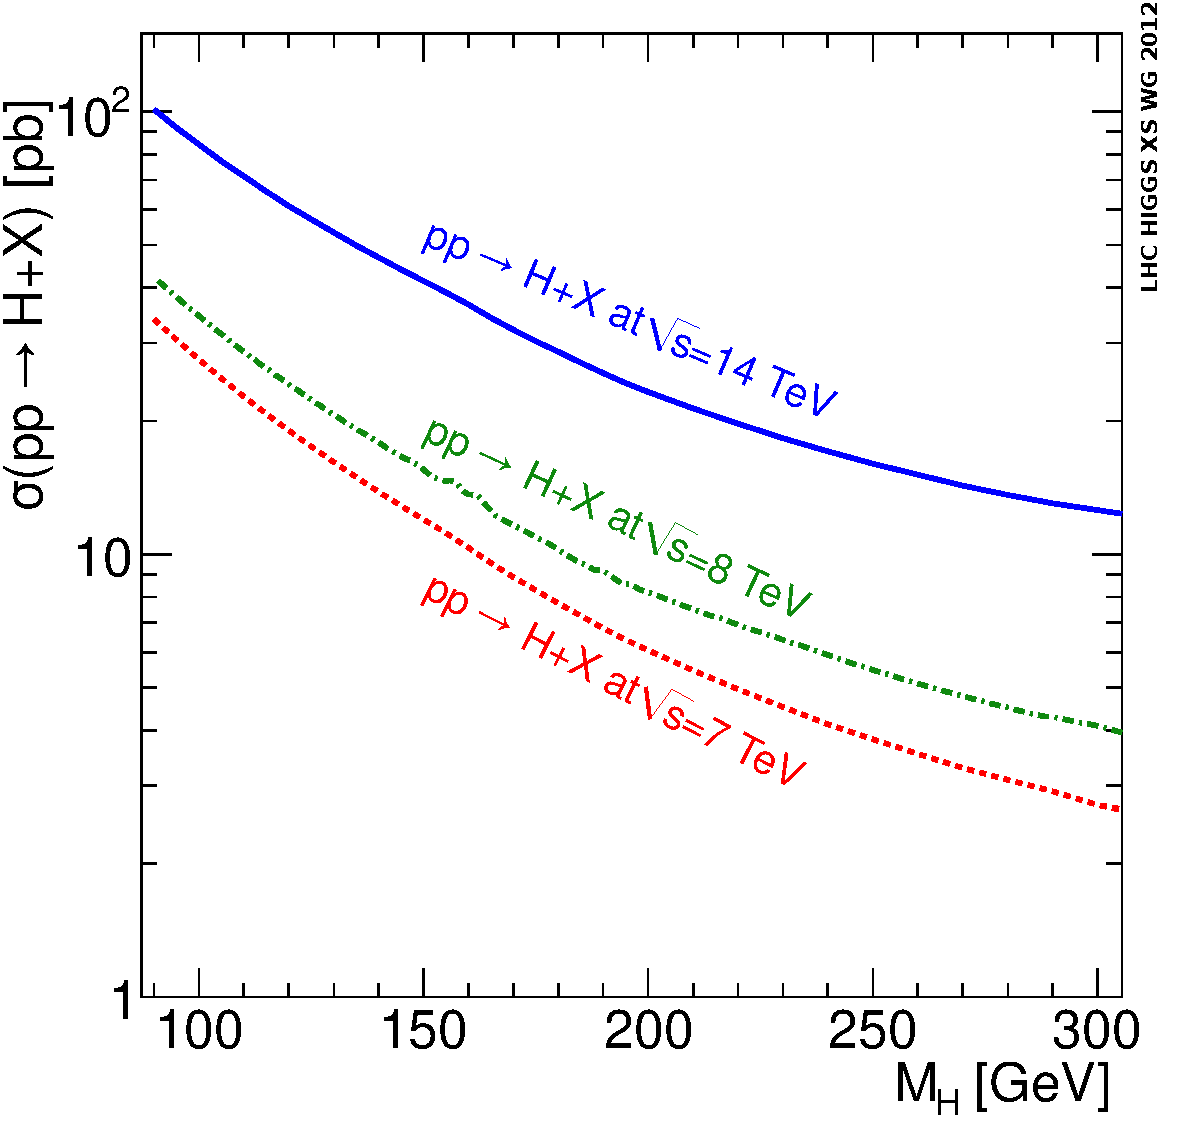
\includegraphics[width=0.5\linewidth]{graphics/totalXS_LM}
	\caption{Total SM Higgs Boson production cross-sections at $\sqrt{s}= 7, 8, 14$ TeV \cite{LHCXSWG_Total_width}}.
	\label{fig:TotalWidth at different TeVs}
\end{figure}

\subsubsection{Gluon-gluon fusion}
\begin{figure}[tb]
	\centering
	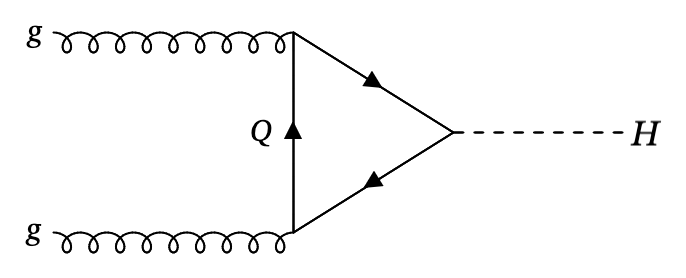
\includegraphics[width=0.5\linewidth]{graphics/gluon_gluon_fusion_LHC}
	\caption{Leading-order Feynman diagram for gluon-fusion Higgs production, via a virtual heavy-quark loop.}
	\label{fig: gluon-gluon fusion}
\end{figure}

With a branching ratio of 58\%\cite{Jones:2023uzh}, the most dominant Higgs production channel at the LHC is gluon-fusion ($gg \rightarrow H$), which is mediated at leading-order, by  a virtual heavy-quark (predominantly top) loop, in the $m_H = $ 115 to 800 GeV range. This channel has the highest branching ratio, and thus, sees more Higgs production events than the other channels; despite this, accessing the dominant Higgs decay channel ($H \rightarrow b\bar{b}$) becomes impossible. Bottom-anti-bottom pairs created via Higgs decay are indistinguishable from the background processes such as direct pair production ($gg \rightarrow b\bar{b}$, $q\bar{q} \rightarrow b\bar{b}$), gluon splitting ($g \rightarrow b\bar{b}$), and higher-order QCD radiation. For $m_H < 150$ GeV, the proposed decay channel is $H \rightarrow \gamma \gamma$, and for $m_H > 2M_Z$ the gold-plated discovery channel is $H \rightarrow ZZ\rightarrow 4\ell$. NLO QCD calculations were computed which boosted the cross-section by roughly 50\% to 100\%; naturally, NNLO corrections were computed in the heavy top limit ($m_t \rightarrow \infty$; consider all quark masses, except for top, and electroweak couplings as negligible), in which the Higgs boson can couple to gluons only via a top quark loop\cite{Kanemura:2018yai}. A comparison to the full NLO correction, up to $m_H = 2m_t$, shows a 5\% agreement; for $m_H > 2m_t$, the difference is only 10\%. NNLO calculations result in a 10\% to 20\% increase above NLO, which implies a perturbative series convergence \cite{Buescher:2005re}.\\


\subsubsection{Vector-boson fusion}

\begin{figure}[tb]
	\centering
	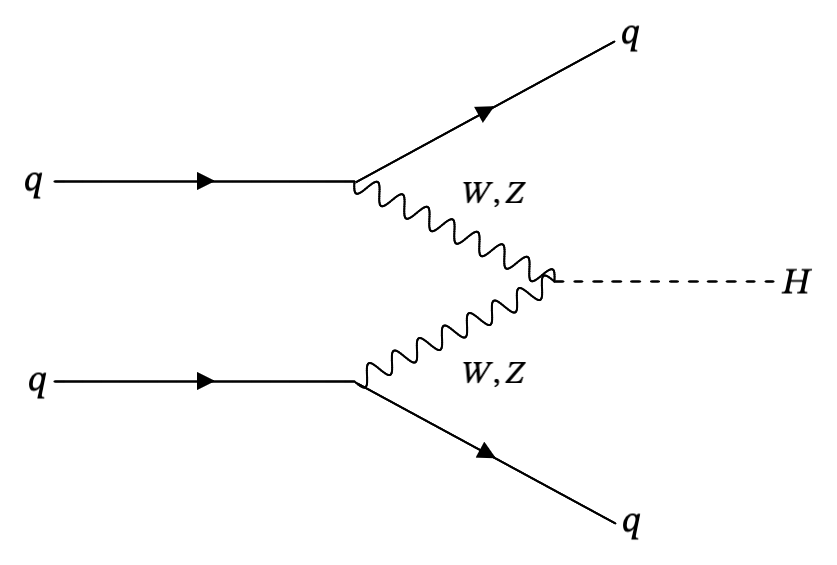
\includegraphics[width=0.6\linewidth]{graphics/VBF_LHC}
	\caption{Leading-order Feynman diagram for Higgs production via vector boson fusion.}
	\label{fig: VBF Feynman}
\end{figure}

With the second-largest cross section (refer to Figure \ref{fig:Width at different TeVs}) for SM Higgs production at the LHC, the vector boson fusion ($qq\rightarrow qqH$) involves incoming quarks  scattering via t-channel exchange of W or Z bosons; the Higgs boson is radiated from the propagator of the exchanged weak boson. Due to the t-channel topology, the scattered quarks remain close to the beam and form forward-backward tagging jets which are ideal for event selection. The exchange of colour-neutral electroweak bosons means that there is no amount of QCD colour flow between the initial and final states, thus, suppresses hadronic activity between the jets. Furthermore, the colour-flow contributions at NLO and NNLO are also suppressed; ultimately, this in conjunction with special VBF selection cuts on the two jets strengthens the VBF signature. The VBF process is known to N$^3$LO QCD + NLO EW accuracy. Before the Higgs discovery in 2012, NLO and NNLO QCD corrections were known: the NLO QCD correction decreased the cross section by 3\% with a $\pm$1\% scale uncertainty and the NNLO QCD correction (calculated using the structure-function approximation \cite{Djouadi:2005gi}) reduced the cross section by 1\% and reduce the scale uncertainty to $\pm$0.5\% \cite{Jones:2023uzh}. The NLO EW corrections decrease the cross section by 5\% \cite{Ciccolini:2007jr}. After 2012, N$^3$LO QCD corrections were found to be between 1 - 2\% and reduced scale uncertainties five-fold \cite{Dreyer:2018qbw}. 

\begin{figure}[tb]
	\centering
	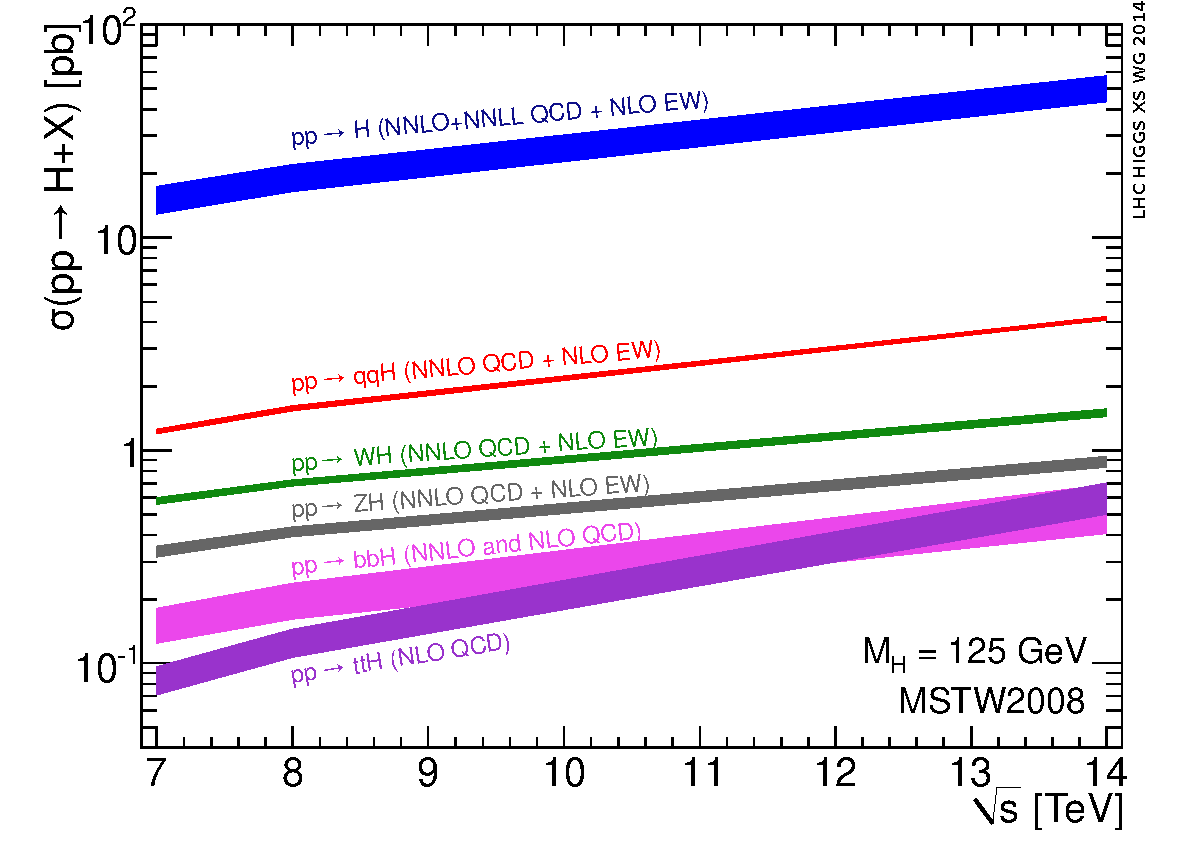
\includegraphics[width=0.6\linewidth]{graphics/7-14.xsec}
	\caption{SM Higgs Boson production channel cross-sections from $\sqrt{s}= 7$ to $\sqrt{s}=14$ TeV \cite{LHCXSWG_Total_width}}
	\label{fig:Width at different TeVs}
\end{figure}




\subsubsection{Production of a Higgs boson with weak gauge bosons/Higgs-strahlung}
\begin{figure}[tb]
	\centering
	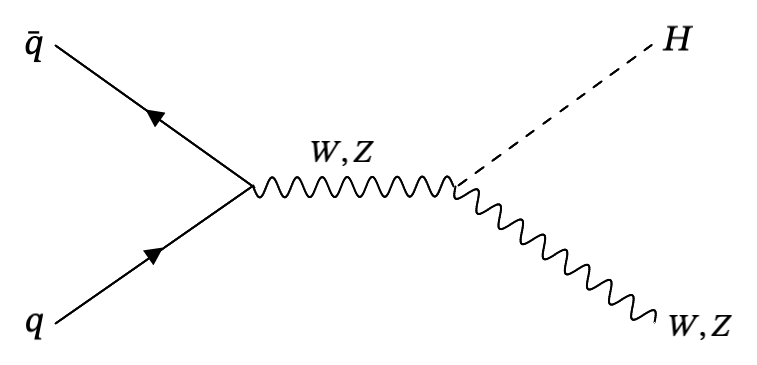
\includegraphics[width=0.6\linewidth]{graphics/Higgsstrahlung_LHC}
	\caption{Leading-order Feynman diagram for Higgs production via Higgs-strahlung mechanism.}
	\label{fig:higgsstrahlunglhc}
\end{figure}


The Higgs-strahlung ($q\bar{q} \rightarrow VH$, $V = W, Z$) is used to probe the light SM Higgs above the LEP limit ($m_H=$ 115 to 130 GeV) at the LHC. The Higgs-strahlung mechanism requires a quark-anit-quark interaction; the LHC is a proton-proton collider, so the required anti-quark must come from the sea, thus, the $q\bar{q} \rightarrow VH$ channel is suppressed relative to gluon-fusion, of which gluons are more abundant. By contrast, at TeVatron the  valence quarks in the proton interact with valence anti-quarks in the anti-proton; the $q\bar{q} \rightarrow VH$ cross-sections are only a few factors below the $gg \rightarrow H$ channel (refer to Figure 1 in \cite{Buescher:2005re}). Consequently, both CDF and D$\phi$ detectors focused their low-mass searches on the $p\bar{p} \rightarrow WH, ZH, t\bar{t}H$ channels. For $m_H < 135$ GeV, the dominant decay mode is $H \rightarrow b \bar{b}$; hadronic decays of W and Z ($W,Z \rightarrow q\bar{q}$) are not preferred as it is hard to distinguish from QCD background processes that produce jets. On the other hand, leptonic decays ($W \rightarrow \ell \nu$ and $Z \rightarrow \ell \ell$) lead to cleaner signals and is the preferred production mode for the $H \rightarrow b\bar{b}$ decay channel. In the 160 GeV to 180 GeV range, the branching ratio of the $H \rightarrow WW $ decay channel is almost 100\% and becomes a viable channel to detect a Higgs via Higgs-strahlung production. The $H \rightarrow\gamma\gamma$ decay channel, despite a small 0.2\% branching fraction \cite{Jones:2023uzh}, has a very clean signature since requiring high transverse-momentum and well-isolated photons and leptons essentially suppresses the irreducible backgrounds, which leads it to be the main detection channel for the Higgs-strahlung production process \cite{Djouadi:2005gi}. At a $\sqrt{s}=14$ TeV LHC, the Higgs production cross-section via Higgs-strahlung gives $\sigma(pp\rightarrow WH) = 1.51$ pb and $\sigma(pp\rightarrow ZH) = 0.98$ pb \cite{LHCHiggsCrossSectionWorkingGroup:2016ypw}. By comparison, at $\sqrt{s} = 1.96$ TeV, TeVatron gives $\sigma(p\bar{p}\rightarrow WH) = 0.13$ pb and $\sigma(p\bar{p}\rightarrow ZH) = 0.079$ pb \cite{TEVNPHTevatronNewPhenomina:2012tcc}. NLO QCD corrections raises the total cross-section by $\sim$ 17\%; NNLO corrections are $\sim 1\%$ and are largely cancelled by NNNLO effects; NLO EW reduces the cross-section by $\sim$ 5\% to 10\%\cite{Jones:2023uzh}. At NNLO, some contribution to the ZH production comes from an effective coupling between the Z-boson and two gluons induces by a quark loop; this accounts for 10\% of the total cross-section\cite{Brein:2003wg}. NLO QCD corrections to this contribution enhances the $gg \rightarrow ZH$  cross-section by 100\%. 

\subsubsection{Production of a Higgs boson with heavy quarks}
\begin{figure}[tb]
	\centering
	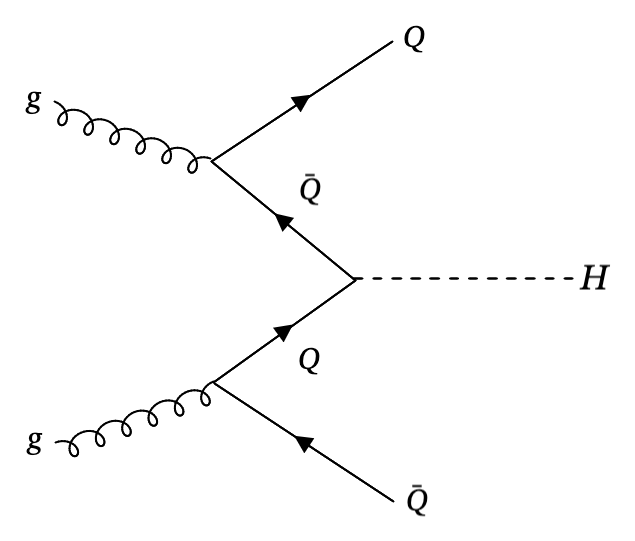
\includegraphics[width=0.6\linewidth]{graphics/Higgs_heavyQ_LHC}
	\caption{Leading-order Feynman diagram for associated Higgs production with heavy quarks.}
	\label{fig:higgsheavyqlhc}
\end{figure}


The top quark plays an important role in the electroweak symmetry breaking mechanism in the SM; indirect evidence for the Yukawa coupling is given by the gluon-gluon fusion channel, given that the process is induced by a top quark loop \cite{Carena:2016hpv}. Unlike gluon fusion, the $t\bar{t}H$ state contains the Yukawa coupling at tree level, therefore, has potential to be a direct probe of the top Yukawa coupling to the Higgs Boson. Experimentally, however, is difficult to measure due to the small cross-section, and vulnerability to irreducible backgrounds. The $t\bar{t}H $ production channel is most efficient for low-mass searches ($m_H < 135$ GeV), thus is naturally most sensitive to the $H \rightarrow b\bar{b}$ decay channel. In the final state $t\bar{t}H \rightarrow WWb\bar{b}b\bar{b}$ (where top and anti-top quarks decay into $W^+$b and $W^- \bar{b}$ respectively), the W-bosons eventually decay to fully leptonic (four leptons), semi-leptonic (two leptons, two quarks) or fully hadronic (four quarks) states. Older simulation studies predicted the $t\bar{t}H$ with $H \rightarrow b\bar{b}$ could serve as a discovery channel in the low-mass range ($m_H \sim$ 80 GeV to 130 GeV) and predicted a signal significance of 5$\sigma$ for $m_H = 120$ GeV with enough luminosity \cite{Sapinski:2000uz}. In reality, the background dominated by $t\bar{t}b\bar{b}$ and also $t \bar{t}W^+$ buries the Higgs signal making it challenging to measure. NLO QCD corrections increased the cross-section by 25\% and the NNLO corrections further increased the cross-section by 4\% at $\sqrt{s}= 13 $TeV\cite{Catani:2022mfv}. NLO EW corrections decreased the cross-section by 1.03\% \cite{Zhang:2014gcy}. \\

The relatively small cross-section coupled with the large backgrounds make the Higgs production in association with b-quarks very difficult to access in hadron colliders. In supersymmetric extensions of the Standard Model, the Yukawa coupling of the b-quark is significantly enhanced; as a result, Higgs production in association with b-quarks can become the dominant production channel. Cross-sections and NLO corrections were calculate through two schemes: the four-flavour scheme presents no b-quarks in the initial state; since gluons can split into b $\bar{b}$ pairs in conjunction with the small b-quark mass, the inclusive cross-section is affected by large logarithmic terms and poor convergence in the perturbative expansion. A way to improve this convergence is via the five-flavour scheme where the logarithms are summed to all orders in the expansion\cite{Buescher:2005re}. \\





\subsection{Higgs Boson Decay}\label{sec: Higgs Decay}
The Standard Model Higgs Boson is unstable and has a short lifetime ($ \approx 1.56 \times 10^{-22}s$) after which it decays into the heaviest kinematically accessible particle-antiparticle pair, with the available decay modes determined by its mass \cite{CMS_life}. Its main decay channels include fermionic modes, bosonic modes, and loop-induced processes and the branching ratios for these channels are also sensitive to the Higgs boson mass. Due to the short lifetime, detection of the Higgs comes from event reconstruction of the decay products; since the the decay products depend on Higgs mass, the detection of certain decay channels set the energy scale for the Higgs Boson. All of the partial decay widths and hence the branching ratio predictions are at NLO (and beyond for $H \rightarrow q\bar{q}$) in both QCD and electroweak perturbation theory, and are calculated using the programmes \verb|HDECAY| and \verb|PROPHECY4F|. \verb|HDECAY| calculates the branching ratio and total decay width for the Standard Model Higgs and the Minimal Supersymmetric extension; all the relevant QCD corrections are included and EW corrections are approximated \cite{Spira:1996if}. \verb|PROPHECY4F| is a Monte Carlo event generator designed to simulate Higgs decays into four-fermion final states via intermediate W or Z bosons and contain only EW corrections \cite{Bredenstein:2006ha}. \\

\subsubsection{Fermionic decay channel}
\begin{figure}[tb]
	\centering
	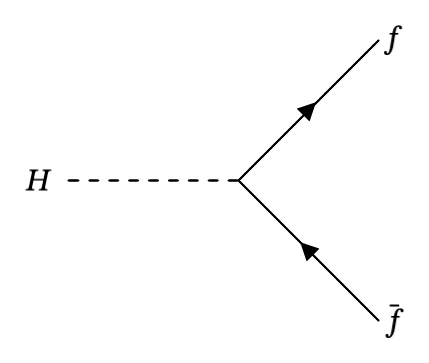
\includegraphics[width=0.4\linewidth]{graphics/H_to_ff}
	\caption{Leading-Order Feynman diagram of SM Higgs Boson decay via fermions.}
	\label{fig:HiggsToff}
\end{figure}

At Higgs masses $\lesssim 140$ GeV, Figure \ref{fig:higgsBR} depicts domination of the fermionic decay channel with the most significant being the $H \rightarrow b \bar{b}$ channel. Due to the relatively heavier mass of the bottom quark, $\sim$ 4.18 GeV \cite{Aparisi_2022}, it's Yukawa coupling to the Higgs field is greater than the other fermions (excluding top); with a branching ratio of 58\%, the SM Higgs to $b\bar{b}$ decay channel is the most dominant Lighter fermionic decays channels are still accessible, yet suppressed \cite{Jones:2023uzh}. In order to predict the partial decay width of the Higgs into quark-anti-quark pairs, the mass of the quark must be chosen with respect to the energy scale  set by the Higgs mass, thus, it is important to derive the Yukawa coupling using the running quark mass rather than its pole mass; using the pole mass naively leads to an overestimate of partial decay widths \cite{Dittmaier:2012nh}. Due to the proportionality of coupling strength to quark mass, implementing running mass is more necessary for heavier quarks such as top or bottom. Further improvements come from applying QCD corrections, which are known up to the fourth-order, and are dominant over Electroweak corrections in the Standard Model\cite{Kanemura:2018yai}.\\ 



\subsubsection{Loop-induced decay channels with massless final state particles}
\begin{figure}[tb]
	\centering
	\begin{subfigure}[b]{0.45\textwidth}
		\centering
		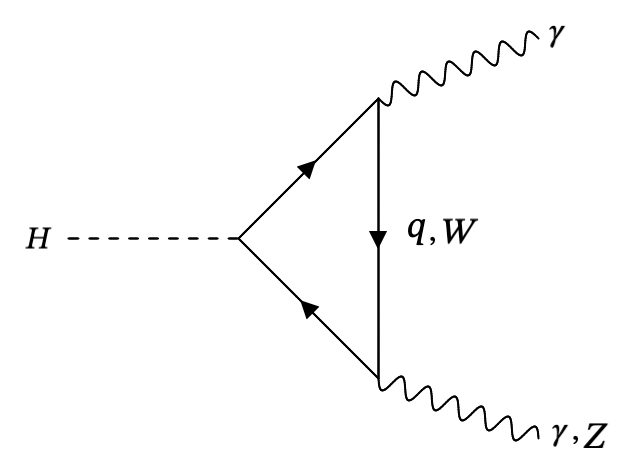
\includegraphics[width=0.9\linewidth]{graphics/Higgs_to_diphoton}
		\caption{Higgs decay to two photons or photon-Z Boson mediated via virtual quark or W-boson loop respectively.}
		\label{fig:H_BR_80_to_200}
	\end{subfigure}
	\hfill
	\begin{subfigure}[b]{0.45\textwidth}
		\centering
		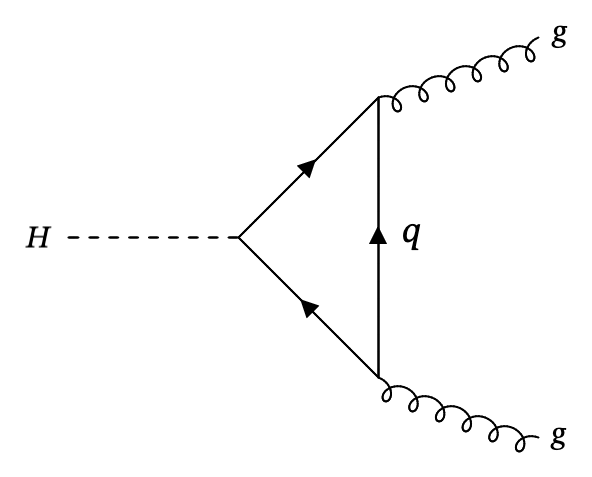
\includegraphics[width=0.9\linewidth]{graphics/gg}
		\caption{Higgs decay to two gluons mediated via a virtual quark loop.}
		\label{fig:BR_YR4}
	\end{subfigure}
	\caption{Leading-Order Feynman diagrams of SM Higgs Boson decay via massless gauge bosons.}
	\label{fig:combined_BR}
\end{figure}



The Higgs Boson has no tree-level coupling to massless gauge bosons. The  $H \rightarrow \gamma \gamma$ decay is mediated via loops of both virtual fermions and virtual W bosons. Gluons only couple to particles that carry colour charge, since W-bosons are colour-neutral, the $H \rightarrow gg$ decay, which accounts for $\sim 8\%$ of the SM Higgs decay \cite{Jones:2023uzh}, is induced only at a virtual quark loop (predominantly the top quark)\cite{Workman:2022ynf}. The NLO QCD corrections to the $H \rightarrow gg$ decay, were initially calculated in the $m_H < 2m_t$ regime, and later for all $m_H$, and adds $\sim$ 40\% to 70\% for $m_H = 100$ GeV to $1$ TeV, to the $H \rightarrow gg$ partial decay width. Additional QCD corrections beyond NLO increase the width by $\sim$ 20\%. EQ NLO add $\sim$ 5\% and mixed QCD-EW contributions are negligible \cite{Dittmaier:2012nh}. The $H \rightarrow \gamma \gamma$ channel sees a relatively smaller number of events (BR $\sim$ 0.2 \% \cite{Jones:2023uzh}) compared to other decay channels. Yet, is important as photons produce well-defined energy deposits in electromagnetic calorimeters which yields highly accurate invariant-mass reconstructions and consequently a narrow resonance peak at the Higgs boson mass\cite{CMS}; this became one of the Higgs Boson discovery channels. The $H \rightarrow \gamma \gamma$ decay was also initially calculated in the $m_H < 2m_t$ regime, and later for all $m_H$. Corrections for small $m_H$ add only $\sim$ 5\% to the partial decay width; for $m_H >2m_t$, corrections can be as large as 50\% to 100\%. The QCD and EW corrections to the $H \rightarrow \gamma Z$ decay are negligible ($\sim$ 1\%) \cite{Reina:2012fs}.\\

\subsubsection{Vector-boson decay channel}
\begin{figure}[tb]
	\centering
	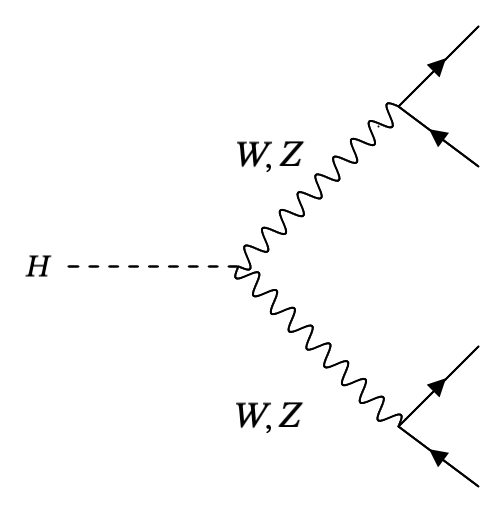
\includegraphics[width=0.4\linewidth]{graphics/higgs_ to_WWZZ}
	\caption{Leading-Order Feynman diagrams of SM Higgs Boson decay via vector gauge bosons.}
	\label{fig:vbflhc}
\end{figure}

The vector-boson decay channel, specifically $H \rightarrow ZZ \rightarrow4 \ell$, serves as another discovery channel for the Higgs Boson. The threshold at which $H \rightarrow WW$ and $H \rightarrow ZZ$ become a fully on-shell decay is when $m_H \geq 160$ GeV and $m_H \geq 180$ GeV respectively, yet, in the region below the 160 GeV threshold, as seen in Figure \ref{fig:higgsBR}, vector-boson decays are significant. A Higgs boson at that energy scale decays via a combination of off-shell and on-shell bosons: $H \rightarrow WW^*$ and $H \rightarrow ZZ^*$ have branching ratios of 21\% and 3\% respectively \cite{Jones:2023uzh}, thus, implies that the vector-boson decay channels are phenomenologically important. Radiative corrections were implemented into \verb|PROPHECY4F| and were calculated using the on-shell masses of the W and Z Boson; the full mass-range was calculated later. For heavy-Higgs-bosons, the decay rate into W and Z bosons increases rapidly, roughly with the cube of the Higgs mass; when $m_H$ approaches 1 TeV, the two-loop corrections become as big as the one-loop correction --- the point at which perturbation theory starts to break down.
\begin{figure}[H]
	\centering
	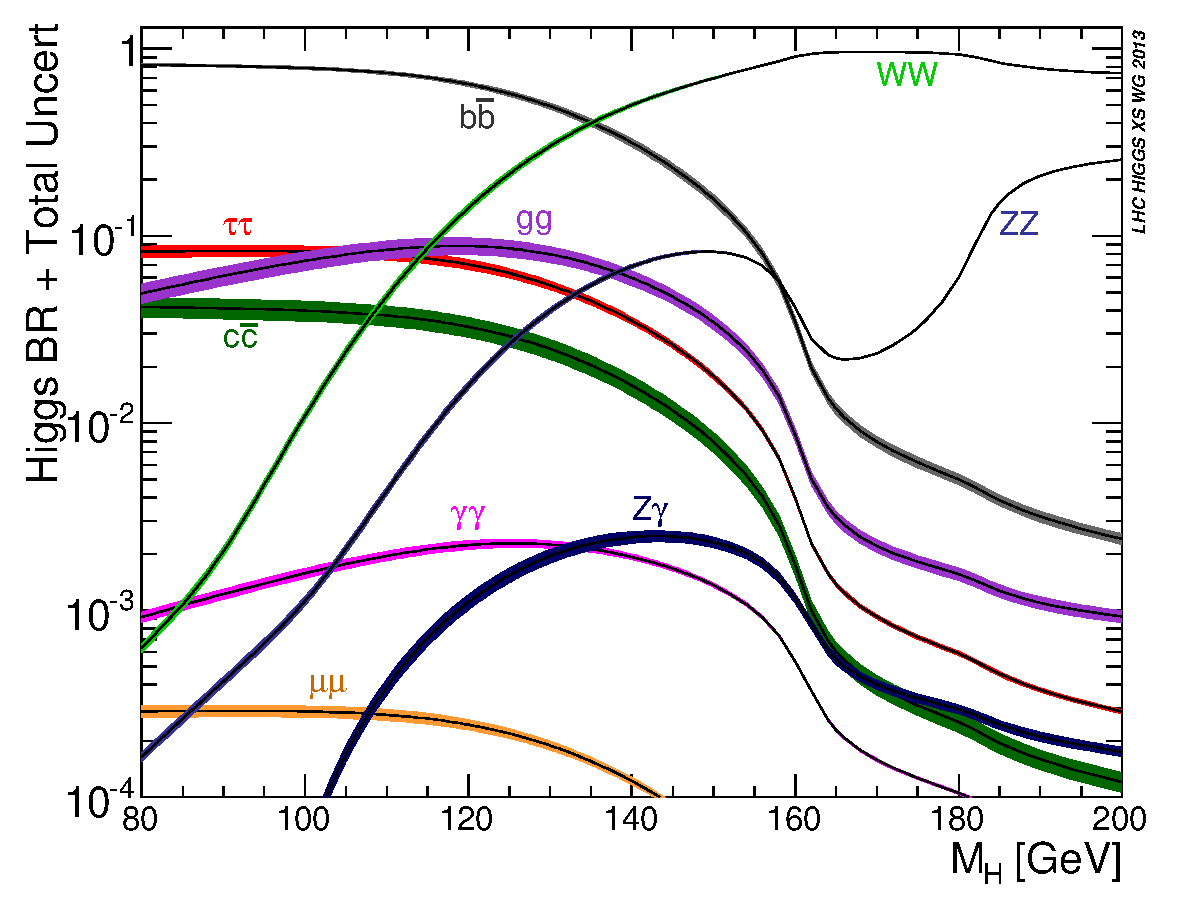
\includegraphics[width=0.6\linewidth]{graphics/Higgs_BR_LM_RECT}
	\caption{SM Higgs Boson branching ratios \cite{LHCXSWG_BR}.}
	\label{fig:higgsBR}
\end{figure}



\section{Higgs boson discovery channels}\label{sec: Higgs Discovery channels}
The discovery channels of the Higgs boson are those decay modes that combine excellent resolution and sufficient sensitivity; amongst the channels discussed in Section \ref{sec: Higgs Decay}, the $H \rightarrow\gamma \gamma$ channel and $H \rightarrow ZZ \rightarrow 4l$ channel (also referred to as the gold-plated channel) provided the cleanest final states, excellent mass and momentum reconstruction, and thus had a significant impact on the discovery of the Higgs boson.\\

Searches in the low-mass region (110 -- 150 GeV) were carried out by both ATLAS and CMS experiments at CERN and included $H \rightarrow$ $\gamma \gamma$, $\tau^- \tau^+$, $b\bar{b}$, $H \rightarrow ZZ \rightarrow l^+l^-l^+l^-$, and $H \rightarrow WW \rightarrow l \nu l \nu$ channels. Despite the low production rate, the $\gamma \gamma$ and $ZZ\rightarrow 4l$ channels offered excellent invariant mass reconstruction; in particular, the barrel section of the electromagnetic calorimeter (ECAL) at CMS achieved an energy resolution of 1\% for photons produced from a Higgs decay event\cite{CMS:2015myp}. The $H\rightarrow WW \rightarrow l\nu l \nu$ channel, on the other hand, had a higher production rate but a full reconstruction was prevented due to the presence of two neutrinos per decay event; only transverse components could be inferred from the measured leptons and missing transverse energy. Similarly, both $\tau^- \tau^+$ and $b\bar{b}$ channels allows partial reconstruction with limited resolution due to the neutrino final states from tau decays and the lack of energy resolution to reconstruct $b\bar{b}$ jets well; no
significant deviation from the background expectation is observed in both channels.\\

With the largest branching ratio in the intermediate-mass region (150 -- 200 GeV), the dominant decay channel was $H\rightarrow WW \rightarrow l \nu l\nu$; as in the low-mass case, only the transverse momentum is reconstructable. The $ZZ \rightarrow 4l$ channel, in this mass region, has a lower production rate that $WW$ but retains excellent mass reconstruction with a resolution roughly one order of magnitude smaller than $H \rightarrow WW$.\\

A range of final states from $WW$ and $ZZ$ decays were considered in the high-mass region (200 - 700 GeV); final state searches by both ATLAS and CMS from the $H \rightarrow ZZ$ decay channel include $ZZ \rightarrow l^+l^-q\bar{q}$, $l^+l^-\nu \bar{\nu}$ and $H \rightarrow WW \rightarrow l\nu q \bar{q}$ --ATLAS only . Semi-leptonic and hadronic decays of the weak-gauge bosons are included to increase signal yields despite the challenging backgrounds; in this mass range, the hadronic decay channels have higher branching ratios relative to regions where $m_H \leq 200$ GeV. These final states are not used in the lower-mass regions because backgrounds from $W/Z$ jets are large and cannot be suppressed sufficiently. For $m_H\geq 350$ GeV, the width of the reconstructed Higgs mass is no longer dominated by experimental constraints but but by the natural Higgs width.

\subsection{$H\rightarrow ZZ $}
\subsubsection{$ZZ \rightarrow \ell^+\ell^- \ell^+\ell^-$}
For Higgs masses between 180 GeV and 700 GeV, the $ZZ^{(*)} \rightarrow \ell^+\ell^-	 \ell^+ \ell^-$ is a reliable candidate for the discovery of the SM Higgs Boson at the LHC. An excess in the invariant-mass spectrum of the four lepton final states ---  $4e$, $4\mu$ and $2e2\mu$ --- over a continuum of  background $Z$ pairs were searched for. Each final state was analysed separately; muons are roughly 200 times heavier than electrons and can traverse thick layers of calorimeters \cite{Muon_spec_ATLAS},  thus are measured differently -  muon momenta are measured in the tracker and the muon detector and electron energy is reconstructed in the electromagnetic calorimeter. Each final state also has its own challenges in identification: signatures from the ECAL come from both real and fake electrons \footnote{Fake electrons refer to particles that detectors and analysis software misidentify as electrons.} produced in background processes such as semi-leptonic decays of heavy quarks, photons coverting into electrons, and jets misidentified as electrons.  \cite{electron_id}; heavy flavour jet decays are a source of fake muons \cite{ATLAS:2020tre}. For ATLAS, the final discriminant is the four-lepton invariant-mass spectrum in which they look for a narrow excess at the Higgs mass ($m_H \approx 125$ GeV) on top of a smooth continuum from background. CMS discriminates further by using the difference in kinematics between the final states. Both ATLAS and CMS experiments saw an excess in the four-lepton invariant mass spectra at $m_H = 125$ GeV and $m_H = 126$ GeV respectively (Figure \ref{fig:hto4l}). 

\begin{figure}[tb]
	\centering
	\begin{minipage}{0.48\textwidth}
		\centering
		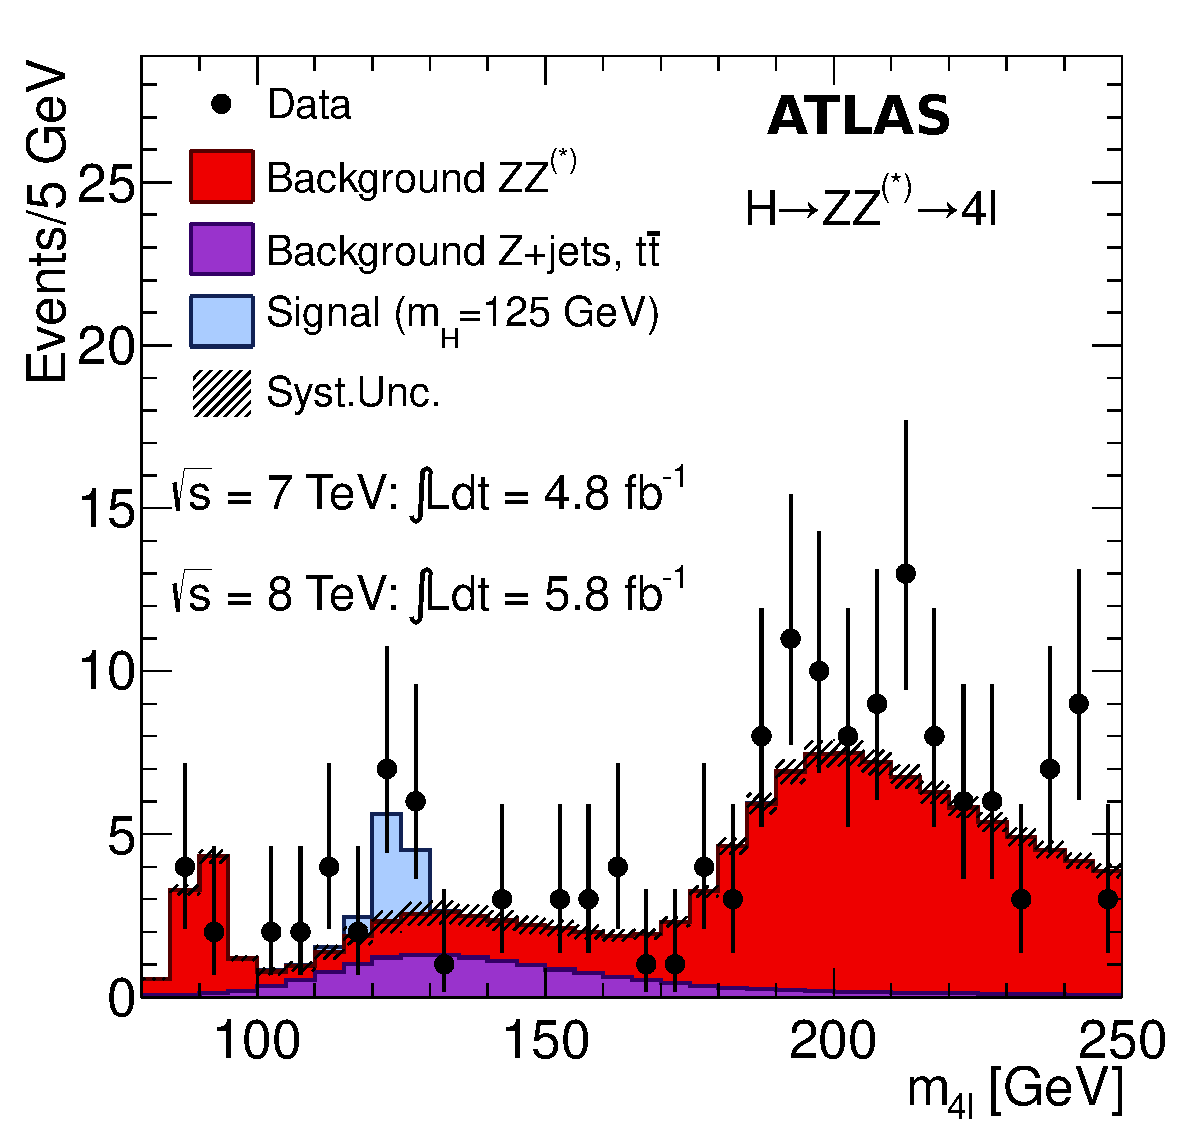
\includegraphics[width=\linewidth]{graphics/atlas_h_zz_4l} 
	\end{minipage}\hfill
	\begin{minipage}{0.48\textwidth}
		\centering
		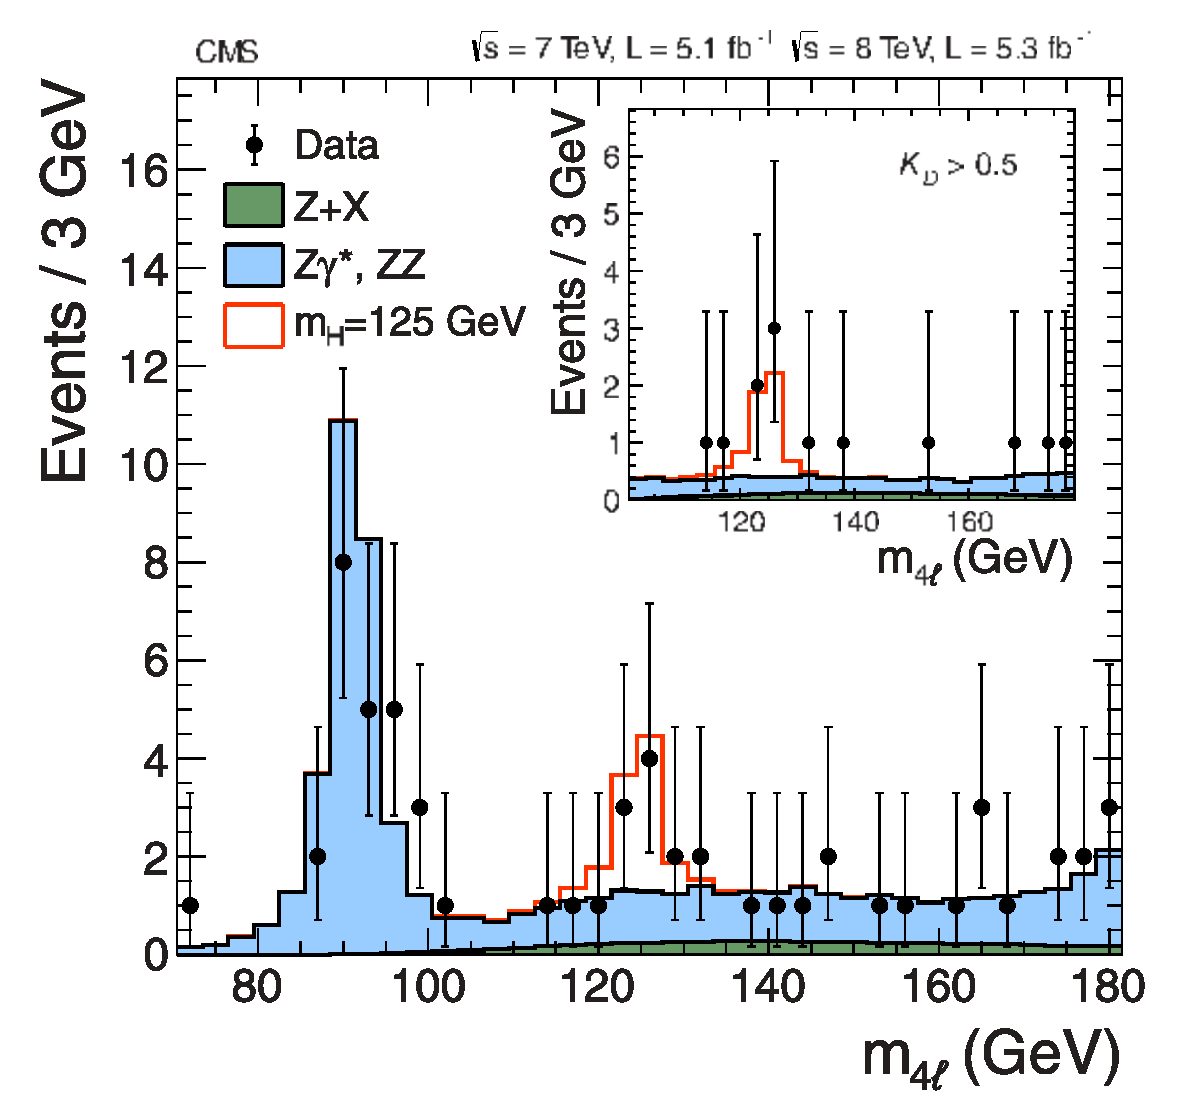
\includegraphics[width=\linewidth]{graphics/cmsh4l} 
	\end{minipage}
	\caption{ATLAS (left) and CMS (right) four-lepton invariant-mass spectra ($H \rightarrow ZZ^{*} \rightarrow 4 \ell$) \cite{Dittmaier:2012nh}}
	\label{fig:hto4l}
\end{figure}
\newpage
\subsubsection{$ZZ \rightarrow \ell^+\ell^- \nu \nu$}
The $H \rightarrow ZZ\rightarrow \ell^+\ell^- \nu \nu$ provides the largest sensitivity in the high-mass range and dominates the sensitivity
for $m_H > 300 $ GeV. The searches require events to contain oppositely charged, same-flavour lepton pairs in conjunction with a large missing transverse momentum - stemming from the pair of neutrinos that are produced in an event. At lower masses, a sizeable proportion of the selected signals come from the $H \rightarrow W^+W^- \rightarrow \ell^+\ell^- \nu \nu$ channel, and so the selection process is designed to avoid double counting of signal yields \cite{Dittmaier:2012nh}.
\begin{figure}[tb]
	\centering
	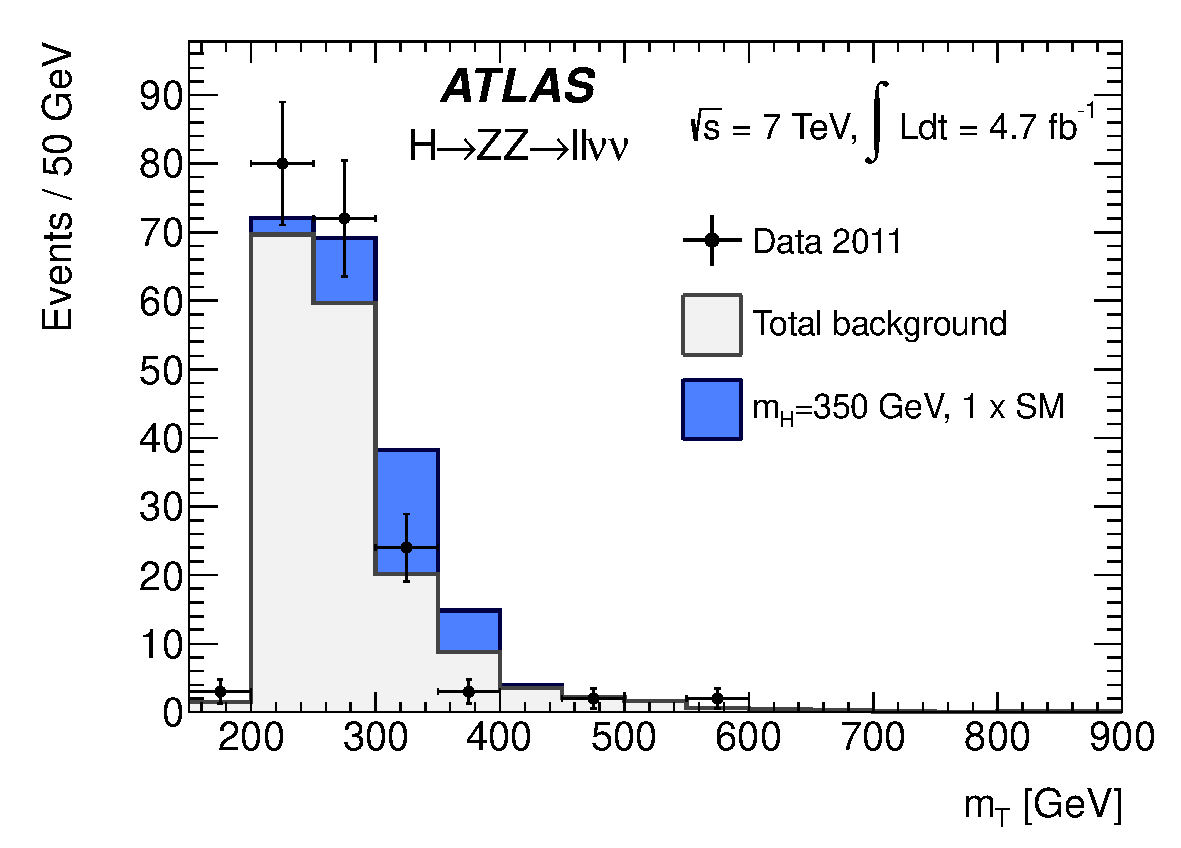
\includegraphics[width=0.6\linewidth]{graphics/atlaszzllnn}
	\caption{Transverse mass, $m_T$, distribution for selected $H \rightarrow ZZ \rightarrow  \ell^+\ell^- \nu \nu$ candidates. Data points (2011) show statistical errors; grey histogram is the predicted background and the blue histogram shows the expected Higgs signal for $m_H= 350$ GeV - if the Higgs was produced at the SM rate. The data is consistent with the background expectation \cite{Dittmaier:2012nh}.}
	\label{fig:atlaszzllnn}
\end{figure}


\subsubsection{$ZZ	 \rightarrow \ell^+\ell^-  q \bar{q}$}
Searches in the $ZZ	 \rightarrow \ell^+\ell^-  q \bar{q}$ channel require an oppositely charged electron or muon pair and a dijet system; in the 
200–700 GeV Higgs-mass range both Z bosons are produced on-shell; consequently the reconstructed invariant masses of the dilepton and dijet systems are required to be consistent with the Z boson mass, $m_Z\approx91.2 $GeV.  The branching ratio for $Z \rightarrow b\bar{b}$ is $(15.12 \pm 0.05) \%$  and is larger than the ratio for $Z \rightarrow \ell \ell$, $(3.366 \pm 0.002)\%$ (refer to table titled "Z Decay Modes" under "Gauge and Higgs Bosons" in \cite{ParticleDataGroup:2022pth}); to exploit this, the decay modes involving b quarks was studied as a means to enhance the signal significance but due to the dominant backgrounds from $t\bar{t}$ and $Zb\bar{b}$ production containing pairs of b-quarks, the discovery sensitivity in this channel is limited (refer to Figure \ref{fig:discriminant_distribution}).
\begin{figure}[tb]
	\centering
	\begin{minipage}{0.48\textwidth}
		\centering
		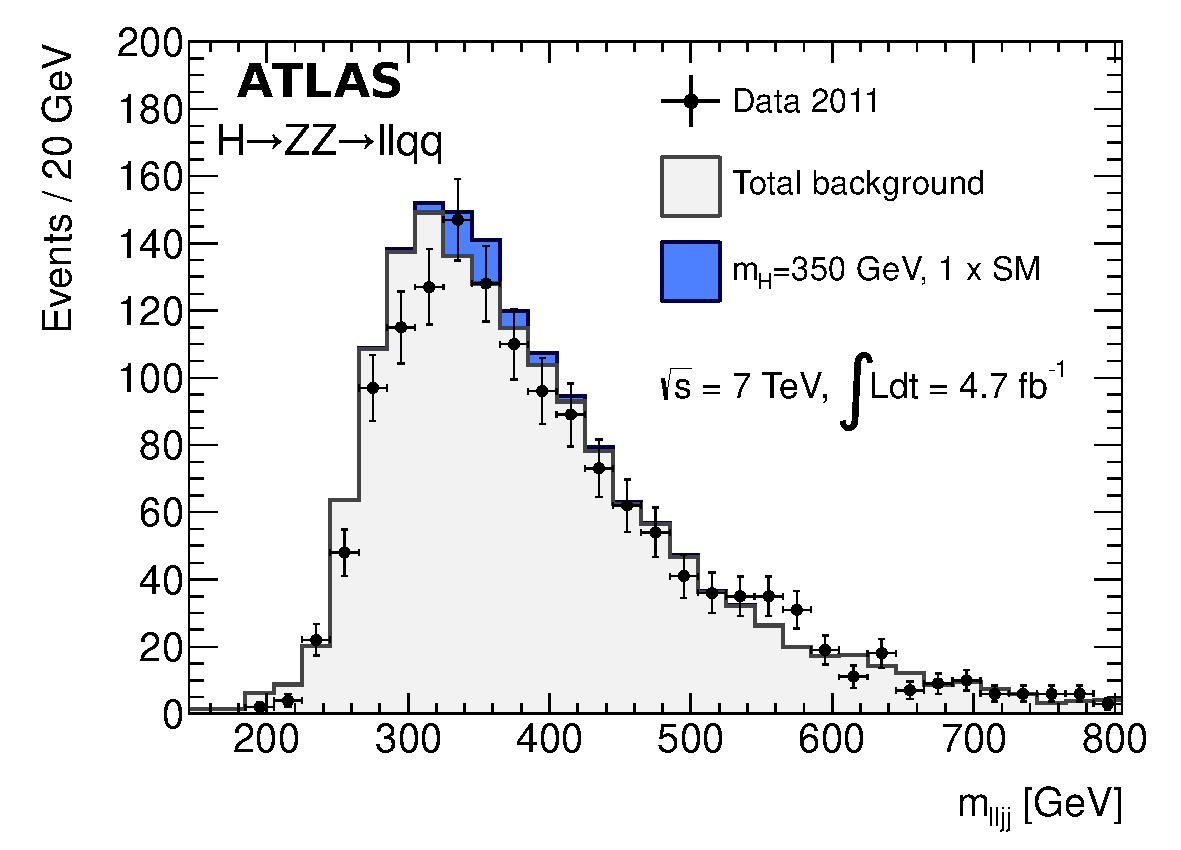
\includegraphics[width=\linewidth]{graphics/atlaszzllqq} 
	\end{minipage}\hfill
	\begin{minipage}{0.48\textwidth}
		\centering
		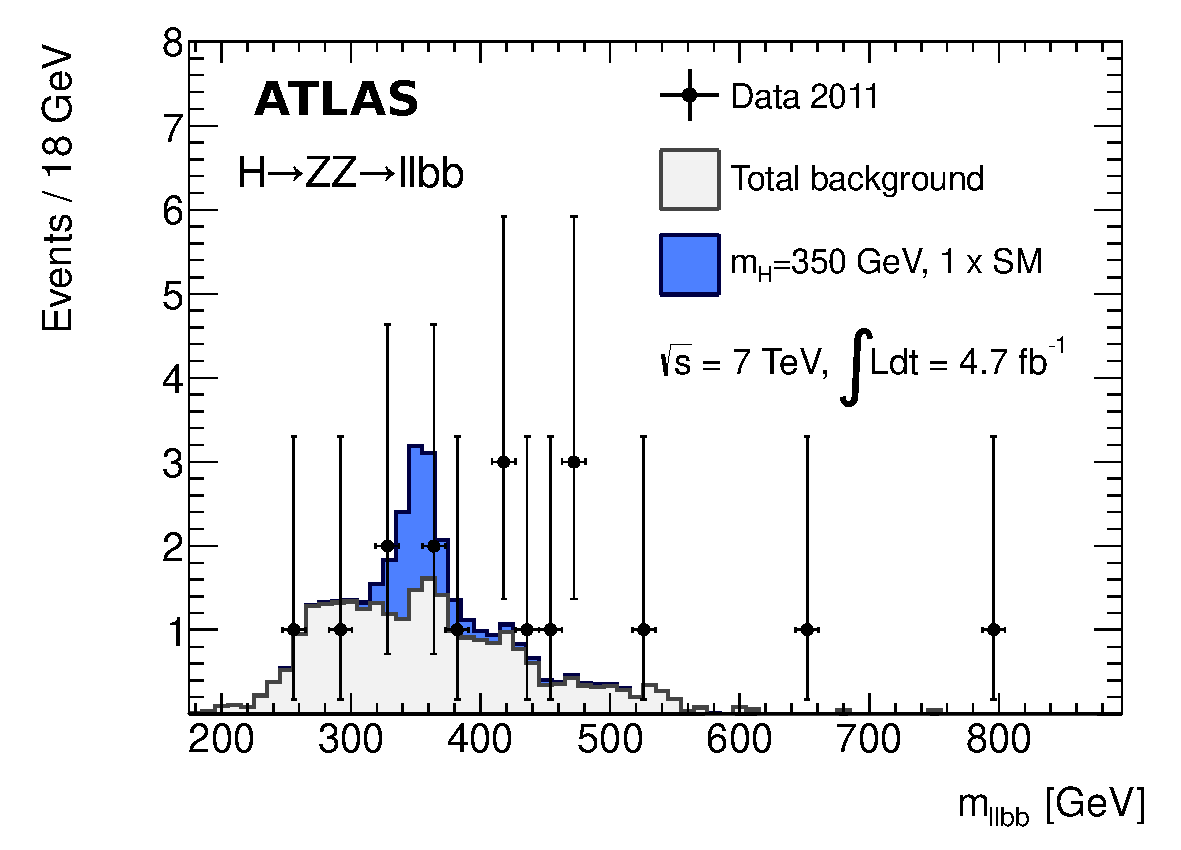
\includegraphics[width=\linewidth]{graphics/atlaszzllbb} 
	\end{minipage}
	\caption{Distributions of the final discriminants for two high-mass Higgs search channels: (left) reconstructed mass, $m_{\ell \ell jj}$, for $H \rightarrow ZZ	 \rightarrow \ell^+\ell^-  q \bar{q}$, (right) reconstructed mass, $m_{\ell \ell bb}$, for $H \rightarrow ZZ	 \rightarrow \ell^+\ell^-  b\bar{b}$.  Data points (2011) show statistical errors; grey histogram is the predicted background and the blue histogram shows the expected Higgs signal for $m_H= 350$ GeV - if the Higgs was produced at the SM rate. The data are consistent with the background expectation within statistical uncertainties \cite{Dittmaier:2012nh}.}
	\label{fig:discriminant_distribution}
\end{figure}


\subsection{$H\rightarrow \gamma \gamma $}
The analysis of the $H \rightarrow \gamma \gamma$ channel focuses on events containing two isolated photons with large transverse momenta and is only detectable in the  80 -- 150 GeV Higgs mass range; the decay events are relatively rare ($\sim 3$ orders of magnitude less than $H \rightarrow b\bar{b}$ in the same mass range; refer to Figure \ref{fig:higgsBR}). There exists a large irreducible background from di-photon production which require excellent energy and angular resolution to observe the narrow mass peak \cite{Buescher:2005re}. A significant challenge arises from the large reducible background due to direct photon production and two-jet events, whose cross sections are several orders of magnitude higher than that of the signal. Fast-simulation studies incorporated smearing of photon polar angle and four-momenta to model the detecor's finite angular and energy resolution; candidates outside the detector’s usable regions are rejected and are accepted only if they are away from other clusters and exist below a threshold of transverse energy inside a cone around them \cite{ATLAS:1999uwa}. These selection criteria show that reducible backgrounds from di-jet and jet-$\gamma$ events can be suppressed to about 20\% of the irreducible prompt $\gamma \gamma$ background across the detectable mass range \cite{Buescher:2005re}.\\

The search's sensitivity is increased by dividing events with different signal-to-background ratios and mass resolutions into categories to be treated separately. Both ATLAS and CMS include a category for the vector boson fusion topology, which is characterised by two extra jets far apart in pseudorapidity which are ideal for event selection. ATLAS further splits events into nine categories. These categories are based on: a photon's pseudorapidity, signatures from unconverted photons, signatures from photons that converted to electron-postiron pairs, and the momentum of the di-photon system transverse to the thrust axis \cite{Dittmaier:2012nh}. CMS instead uses four categories defined by the output score of a boosted decision tree. Both experiments see a clear excess in that spectrum — peaking at about 126 GeV in ATLAS and 125 GeV in CMS (see Figure \ref{fig:atlas_cms_diphoton}).


\begin{figure}[tb]
	\centering
	\begin{minipage}{0.50\textwidth}
		\centering
		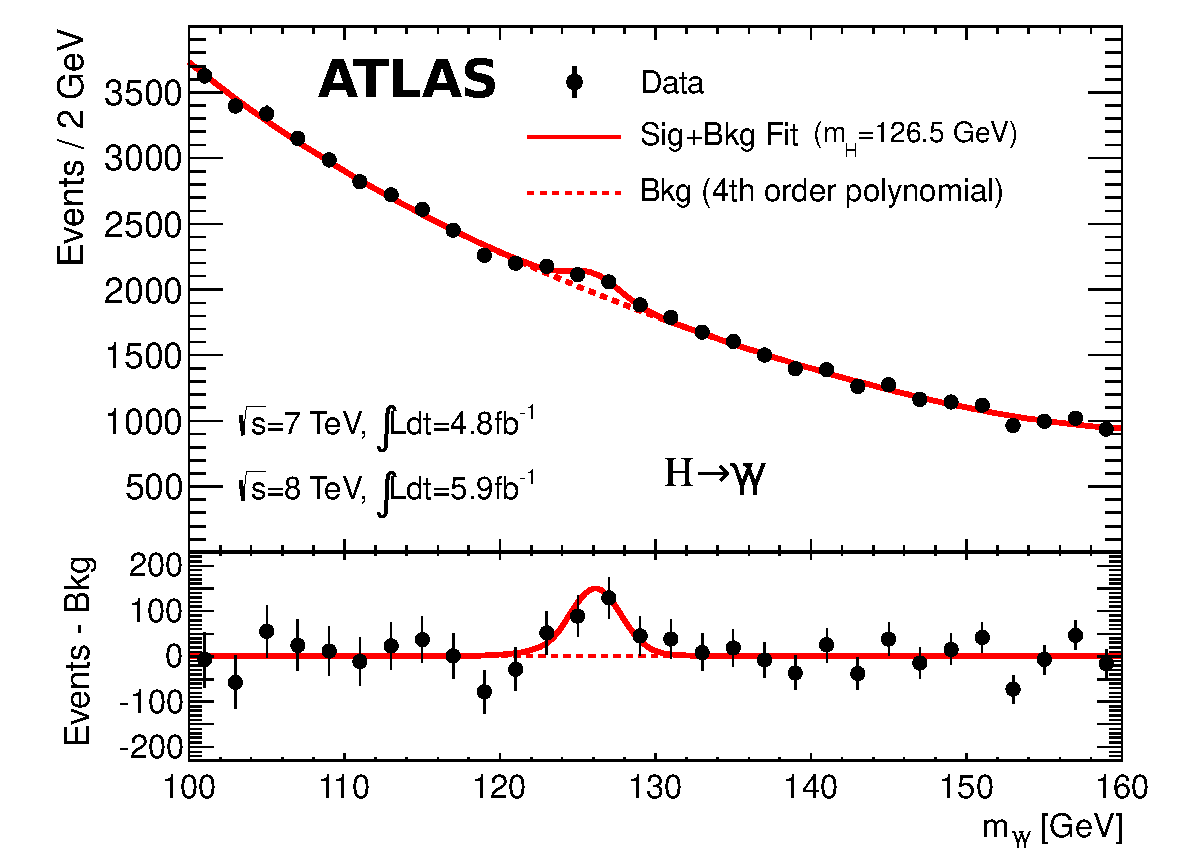
\includegraphics[width=\linewidth]{graphics/atlashgg} 
	\end{minipage}\hfill
	\begin{minipage}{0.45\textwidth}
		\centering
		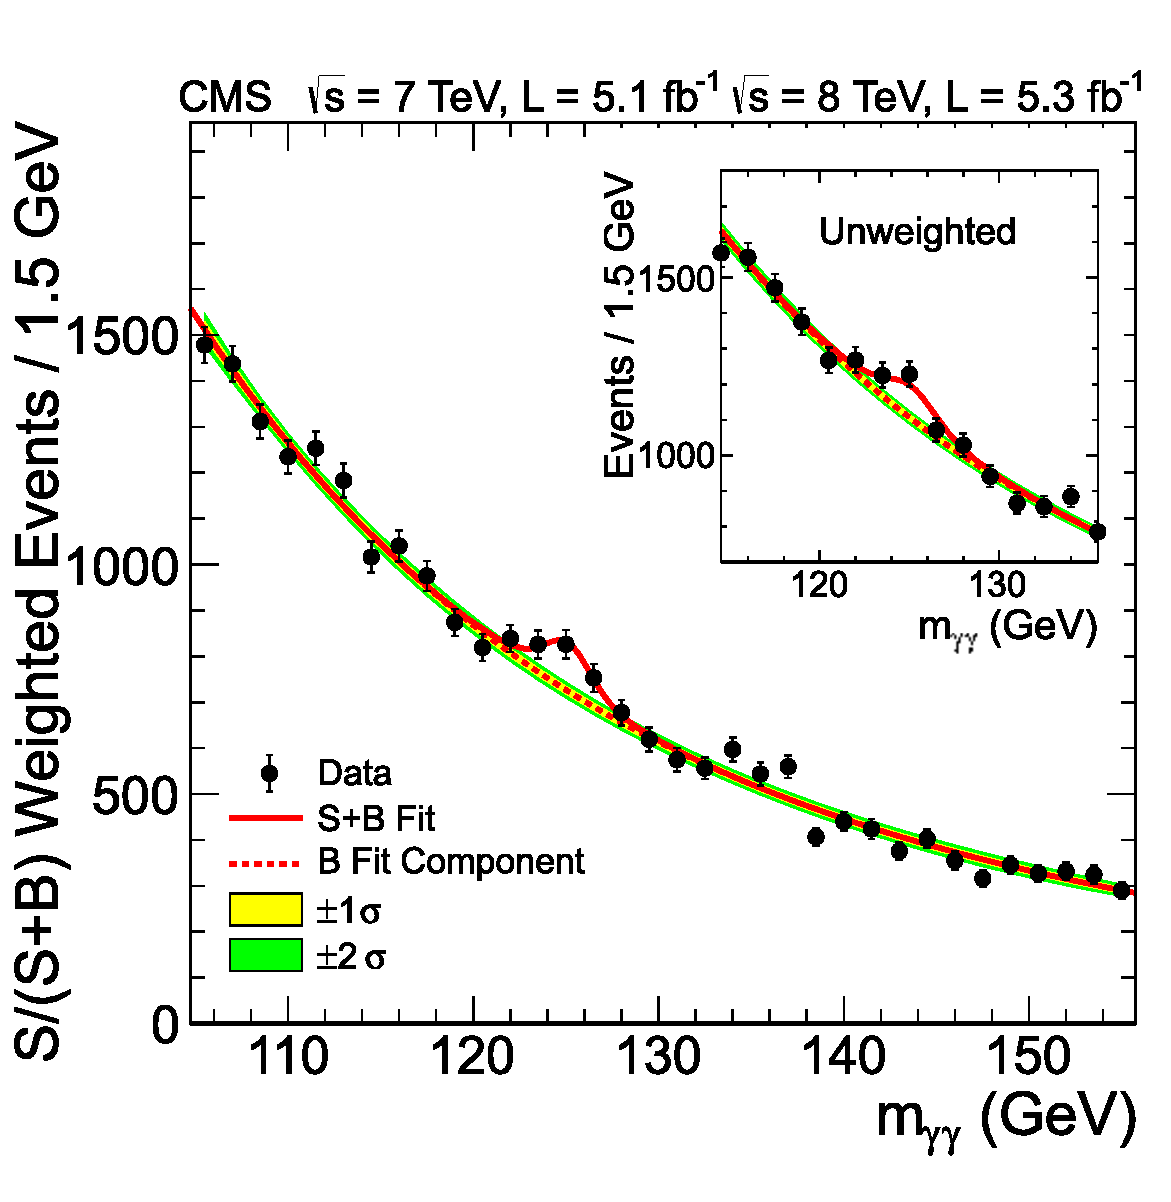
\includegraphics[width=\linewidth]{graphics/cmshgg} 
	\end{minipage}
	\caption{Di-photon invariant-mass spectra after the inclusive selection for the combination of 2011 and 2012 data, shown separately for ATLAS (left) and CMS (right). The two distributions illustrate an excess in the di-photon mass region around 125–126 GeV above the smooth background expectation, as observed in both experiments\cite{Dittmaier:2012nh}.}
	\label{fig:atlas_cms_diphoton}
\end{figure}




\subsection{$H\rightarrow W^+W^- $}
\subsubsection{$H \rightarrow W^+W^- \rightarrow \ell^-\bar{ \nu} \ell^+ \nu $}
For $m_H \geq 160$ GeV --- where ZZ branching ratio is suppressed --- searches in the  $H \rightarrow W^+W^- \rightarrow \ell^-\bar{ \nu} \ell^+ \nu $ decay channel can enhance discovery potential; analysis focuses on excess events with two leptons of opposite charge and large missing transverse momentum. As it is not possible to reconstruct a Higgs mass peak with this channel due to the presence of neutrino final states, the excess of events above the expected backgrounds is used to establish the presence of a Higgs boson signal.	Similar to analysis in the $H \rightarrow \gamma \gamma$ channel, events are split into categories in accordance with lepton flavour and number of jets; events with two jets have selection criteria designed to enhance sensitivity to the VBF production process \cite{Dittmaier:2012nh}. Events with no-jets, the dominant background comes from WW scattering events without a massive particle mediating the process (non-resonant); one-jet events have WW and top-quark production as the main background and two-jet events have top-quark production as the main background. The distribution of the WW transverse mass ($m_W$) for ATLAS and di-lepton invariant mass ($m_{\ell \ell}$) for CMS in the analysis of 8 TeV data show a clear broad excess in ATLAS and a less significant broad one in CMS (see Figure \ref{fig:atlas_cms_ww_lvlv}).
\begin{figure}[tb]
	\centering
	\begin{minipage}{0.50\textwidth}
		\centering
		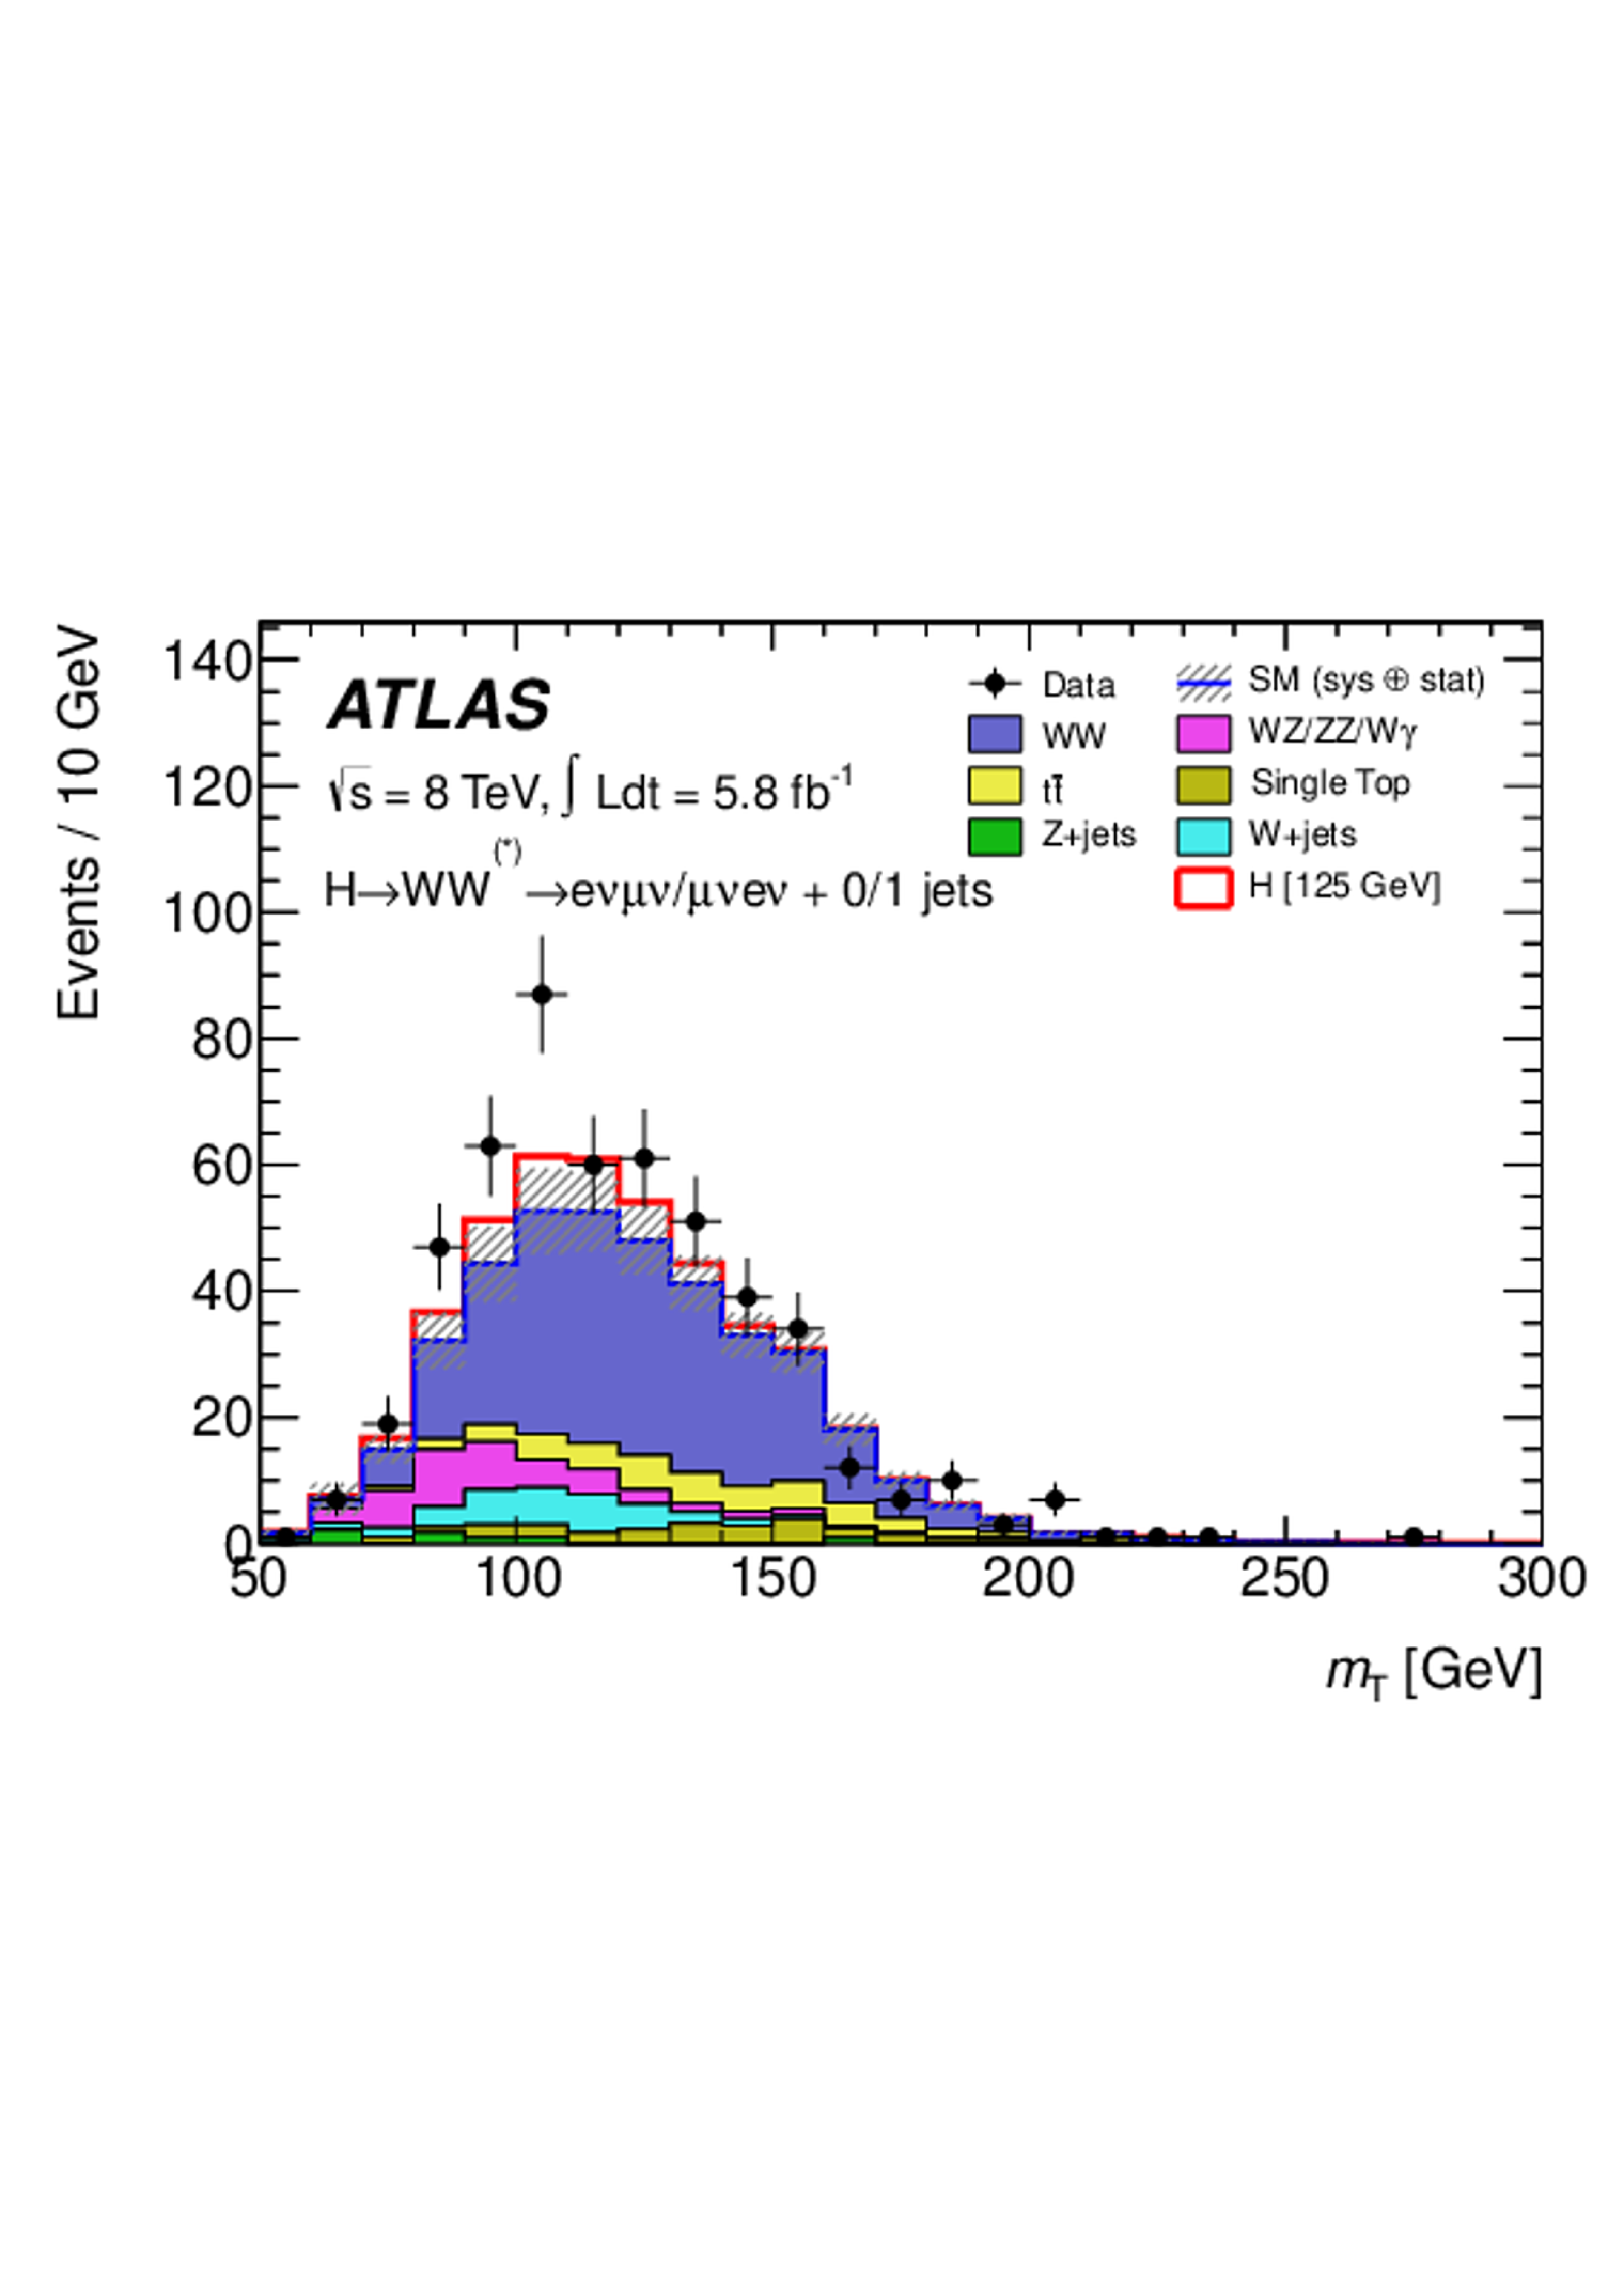
\includegraphics[width=\linewidth]{graphics/atlaswwllnn8} 
	\end{minipage}\hfill
	\begin{minipage}{0.45\textwidth}
		\centering
		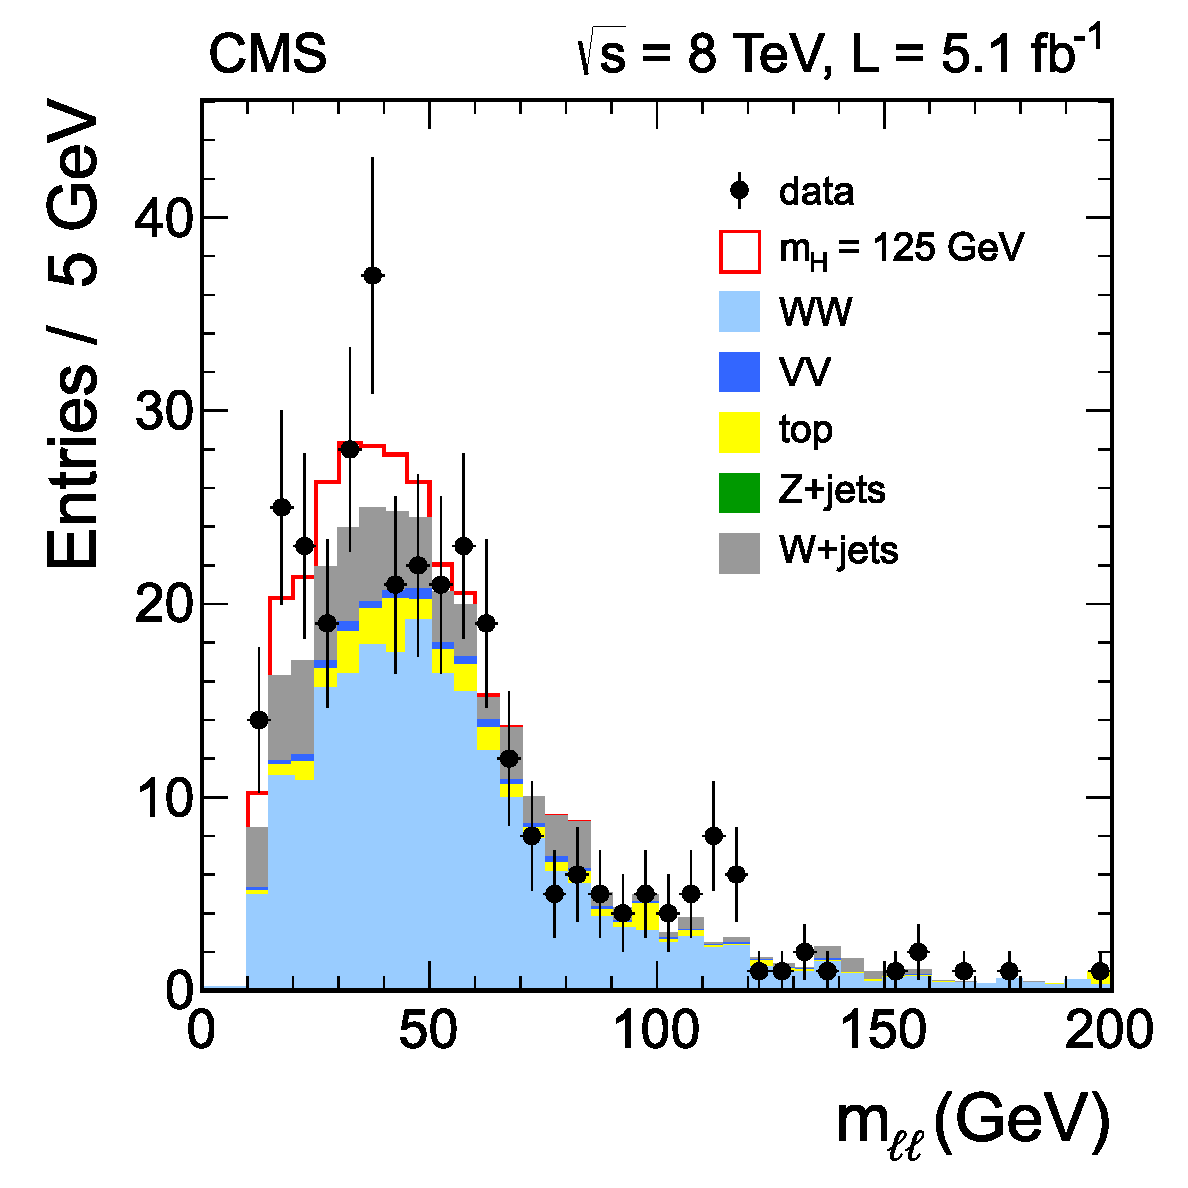
\includegraphics[width=\linewidth]{graphics/cmswwllnn8} 
	\end{minipage}
	\caption{WW transverse mass and di-lepton invariant-mass distributions at $8$ TeV using 2012 data, shown separately for ATLAS (left) and CMS (right). The plots compare the observed data to the predicted SM backgrounds and highlights where a SM Higgs boson of $m_H = 125$ GeV would appear in the $H\rightarrow WW \rightarrow \ell^-\bar{ \nu} \ell^+ \nu$ search\cite{Dittmaier:2012nh}.}
	\label{fig:atlas_cms_ww_lvlv}
\end{figure}

\subsubsection{$H \rightarrow W^+W^- \rightarrow \ell \nu q \bar{q} $}
The $H \rightarrow W^+W^- \rightarrow \ell \nu q \bar{q} $ --- analysed by ATLAS only --- provides additional discovery potential for a heavy Higgs boson ($m_H\gtrapprox 800$ GeV); the analysis requires events with isolated leptons, missing transverse momentum, and two jets with an invariant mass comparable to the W boson. The $\ell \nu q \bar{q}$ final state benefits from the large hadronic W branching fraction ($\sim 10^2$ orders of magnitude higher than $ZZ\rightarrow 4\ell$ at $\sqrt{s}= 8$ TeV -- refer to Figure \ref{fig:hdecaydecay}), thus has a greater signal yield; this channel contains larger reducible and irreducible backgrounds, and poorer mass resolution due to the presence of a neutrino in the final state. Vector boson fusion is an important production mechanism for this channel and therefore for heavy Higgs searches; VBF events produce two final state quarks separated by a large rapidity gap which provides an additional signature for isolating signal from background \cite{Buescher:2005re}. Similar to the analyses of the $H \rightarrow \gamma \gamma$ and $H \rightarrow WW$ channels, the events are split into categories in accordance of lepton flavour and number of jets; the di-jet final state is designed to exploit the VBF topology. This channel has high yield, and compliments searches alongside other  channels, but because the signal is broad and backgrounds are large (refer to Figure \ref{fig:atlaswwlnqq}), it does not provide sufficient evidence for a standalone discovery. 
\begin{figure}[tb]
	\centering
	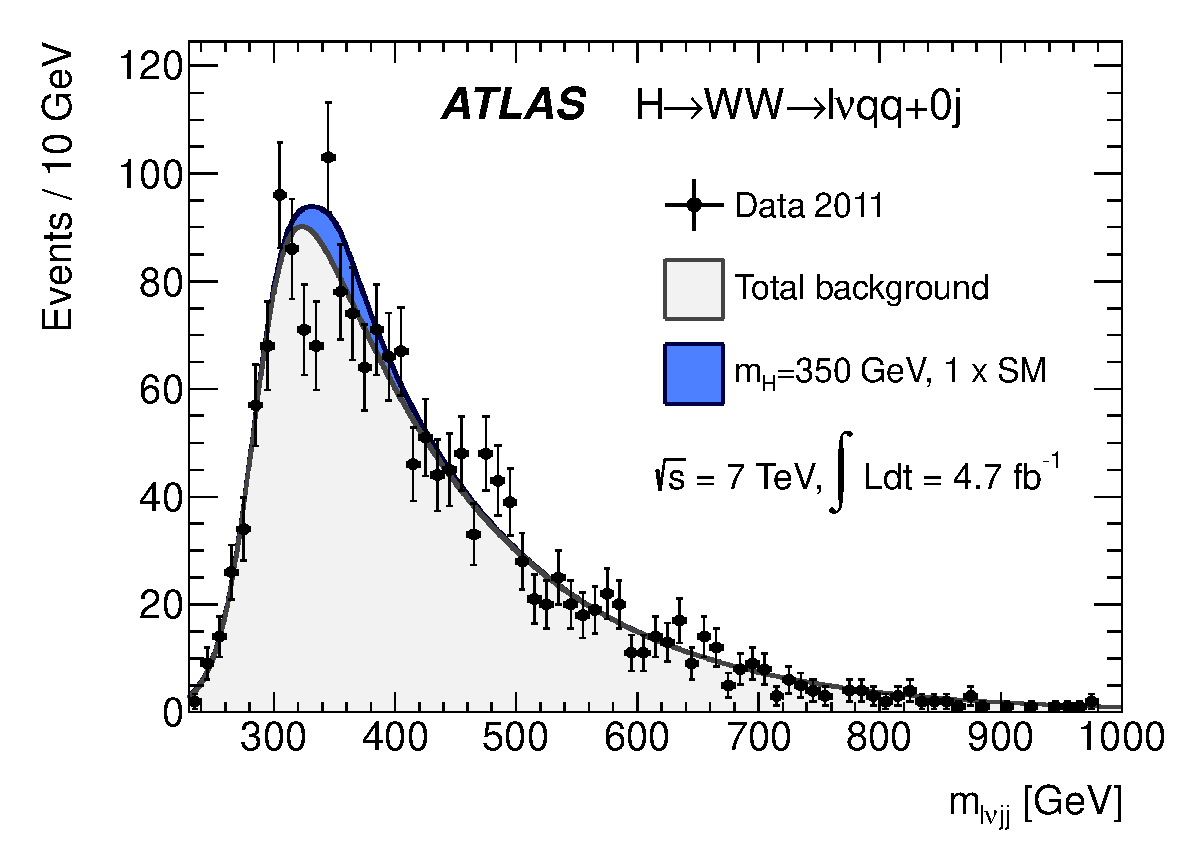
\includegraphics[width=0.6\linewidth]{graphics/atlaswwlnqq}
	\caption{Distribution of reconstructed Higgs candidate mass, $m_{\ell \nu j j}$,  at 7 TeV. Observed data points show statistical errors; grey histogram is the total predicted background and the blue histogram shows the expected Higgs signal for $m_H= 350$ GeV - if the Higgs was produced at the SM rate. No significant excess above the background fit is visible; the plot demonstrates the channel’s high yield but comparatively low signal-to-background and poorer mass resolution relative to fully leptonic modes\cite{Dittmaier:2012nh}.}
	\label{fig:atlaswwlnqq}
\end{figure}


\begin{figure}[tb]
	\centering
	\includegraphics[width=0.5\linewidth]{graphics/h_decay_decay}
	\caption{Standard Model Higgs boson production cross section times branching ratio as a function of Higgs mass ($m_H$) at 8 TeV \cite{LHCXSWG_Total_width}.}
	\label{fig:hdecaydecay}
\end{figure}



\section{Higgs boson searches using vector boson fusion}
Preforming a search for Higgs boson production, across intermediate to high-mass ranges, in the vector boson fusion mode provides a significant increase in discovery potential. At leading order, VBF contributes $\sim 20\%$ of the total Higgs production cross-section, yet it's event topology --- namely, tag jets with large pseudorapidity and suppression of central jet activity --- can be exploited to suppress backgrounds. In vector boson fusion events, the Higgs boson is produced alongside two forward tag jets originating from the scattered initial-state quarks. The scattered quarks emit W or Z bosons, thus, t-channel VBF events proceed via colour-singlet\footnote{W,Z bosons are colour-singlets, i.e. they carry no colour due to the colour-singlet field being a trivial representation of SU(3) --- remains the same under an SU(3) rotation.} exchange at leading order. Therefore, QCD radiation between those tag jets is suppressed, resulting in reduced hadronic activity in the central detector. Requiring two forward tag jets while suppressing  hadronic activity in the central rapidity region exploits the VBF colour-singlet topology and greatly suppresses QCD backgrounds, which ultimately improves the signal-to-background ratio. Jets with the highest transverse momentum in the positive and negative regions of pseudorapidity are chosen to be the tag jet candidates and each jet is required to have a transverse energy of at least 20 GeV \cite{Buescher:2005re}. Subsequent sections detail the analysis of Higgs boson production via vector boson fusion for multiple decay channels.	

\subsection{$qqH \rightarrow qqWW^{(*)}$}
According to parton level simulation studies, the $H \rightarrow WW^{(*)} \rightarrow \ell^+ \ell^- p^{miss}_T $ was found to be a promising discovery channel for the mass range $m_H= 140$ -- $190$ GeV; the distinctive signature leads to a signal-to-background ratio greater than 1 --- which is better compared to the inclusive $H \rightarrow WW^{(*)}$ channel, which is dominated by the gluon fusion process \cite{Buescher:2005re}. Backgrounds are strongly suppressed by identifying the tagging jets associated with WW-fusion \cite{Buttar:2002oza}. After selection cuts,  the expected signal cross-section in the $e\mu$ channel for a Higgs boson with a mass of $160$ GeV is on the order of 4.6 fb above a total background expectation of 1.2 fb \cite{Buescher:2005re}. Given the large signal-to-background ratio, this channel provides strong discovery potential for a Higgs boson near $160$ GeV.\\

The distribution of $\Delta \phi$ (the difference in azimuthal angle between the two leptons in the final state) can also be used to demonstrate the presence of a signal. Figure \ref{fig:delphi} shows the distribution of $\Delta \phi$ for $e\mu$ final states; the events are split into a signal sample ($M_T  <  175$ GeV) and a control sample ($M_T > 175$ GeV). A peak can be seen at small $\Delta \phi$  in the signal sample --- typical behaviour for a scalar particle decay process. On the other hand, this behaviour is not seen for events in the control sample, where WW and $t\bar{t}$  backgrounds dominate.\\

Studies have been done to exploit the larger branching ratio of the hadronic decay of the W boson originating from a VBF process:$qq \rightarrow qqH \rightarrow qqWW^{(*)} \rightarrow qq \ell \nu qq$. The signal cross section multiplied by the branching ratio is approximately 4.3 times larger than in the dilepton channel. However, the W produced in association with background jets share the same final states as the signal, which contribute to the background that ultimately leads to a cross-section more than two orders of magnitude larger than the signal cross section \cite{Buescher:2005re}. This channel is not a suitable candidate for a Higgs boson discovery  but could be used to confirm an observation of a Higgs boson with a mass $\sim 160 $ GeV.\\

The $qq \rightarrow qqH \rightarrow WW \rightarrow \ell \nu \ell \nu$ has been used in combination with other decay channels, to increase the Higgs boson discovery potential in the high mass region between 300 GeV and 600 GeV \cite{Dittmar:2001ifa}.

\begin{figure}[tb]
	\centering
	\begin{minipage}{0.48\textwidth}
		\centering
		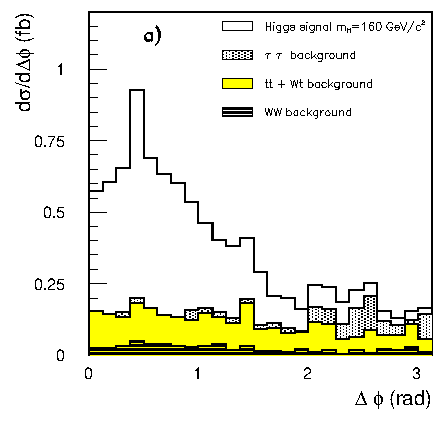
\includegraphics[width=\linewidth]{graphics/vbf_delphi1} 
	\end{minipage}\hfill
	\begin{minipage}{0.48\textwidth}
		\centering
		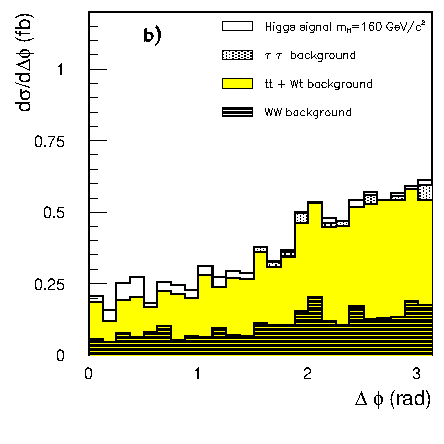
\includegraphics[width=\linewidth]{graphics/vbf_delphi2} 
	\end{minipage}
	\caption{Distributions of $\Delta \phi$,  the difference in azimuthal angle between the two leptons in the final state,  for events in the signal
		region ($M_T < 175$ GeV --- left) and events outside the signal region ($M_T > 175 $GeV --- right) \cite{Asai:2004ws}.}
	\label{fig:delphi}
\end{figure}

\subsection{$qqH \rightarrow qq\tau \tau $}
The ATLAS and CMS experiments are sensitive to the $qqH \rightarrow qq \tau \tau$ channel in the mass region $110 < m_H <140$ GeV \cite{Buescher:2005re}. Searches for $H\rightarrow \tau \tau$ were done using the double leptonic decay mode and the lepton-hadron decay modes, where the Z boson decays to a tau pair constitutes the principal background. In these signal and background events, H and Z bosons are produced with a large transverse momentum, which the tau pairs inherit, and leads to the tau decay products being almost collinear in the lab frame. Under the assumption that the tau directions are given by the directions of the visible tau decay products, the $\tau \tau$ invariant mass can be reconstructed using the collinear approximation. A discovery based on a combination of these final states would require an integrated luminosity of about 30 fb$^{-1}$, assuming the $Z \rightarrow \tau \tau $ background in the signal region is known with a precision of $\pm$10$\%$ \cite{Buescher:2005re}. The $H \rightarrow \tau \tau$ decay is important for measurements of the tau Yukawa coupling to the Higgs field and Higgs boson searches in MSSM scenarios.


\subsection{$qqH \rightarrow qq\gamma \gamma$}
The $H \rightarrow \gamma \gamma $  decay channel has a small branching ratio --- approximately 3 orders of magnitude less than $H \rightarrow WW$ for a 125 GeV Higgs --- so the expected signal rate in the VBF channel is small. Backgrounds include non-resonant $\gamma \gamma$ production in association with jets ($\gamma \gamma j j$), QCD multijet ($jjjj$) and direct photon production. VBF searches typically require tagging jets with a large separation in pseudorapidity, which helps suppress many backgrounds, but due to the rarity of the signal, small background rates are important and considered. After relevant selection and assuming an integrated luminosity of 30 fb$^{-1}$, a signal significance of $2.2 \sigma$ for a Higgs mass of 130 GeV was found \cite{Buescher:2005re}.

\subsection{$qqH \rightarrow qqZZ^{*}$}
For Higgs masses above the kinematic threshold  $m_H > 2m_Z$, the $ZZ \rightarrow \ell \ell qq$ --- in which one Z boson decays leptonically to a same-flavour opposite-sign lepton pair and the other decaying hadronically to two quarks (reconstructed as jets) ---  is studied. Unlike the fully leptonic ($ZZ \rightarrow 4 \ell$) final state, $\ell \ell qq$ benefits from a larger branching ratio, yet, is dominated by $Z+4$jet backgrounds. For a $m_H = 350$ GeV Higgs, a signal significance of $3.8 \sigma$ has been estimated, assuming an integrated luminosity of 30 fb$^{-1}$, which is weaker than that of the $H \rightarrow 4 \ell$ channel \cite{Buescher:2005re}. 

\subsection{$qqH \rightarrow qqb  \bar{b}$}
Given the large background from QCD jet production, searches in the $qqH \rightarrow qqb  \bar{b}$ is challenging. The LO QCD background for the $H \rightarrow b \bar{b}$ process is large, even after imposing the presence of rapidity gaps and the high transverse momentum cuts \cite{DeRoeck:2002hk}. According to parton-level simulations, the 4-jet final state background is over 100 times larger than the signal. A large contribution comes from two separate proton–proton collisions that overlap in the same bunch crossing. The overlapping events produce a $b\bar{b}$ mass distribution with a broad peak that sits in the middle of the signal region, thus contaminating the Higgs peak \cite{Mangano:2002wn}. However, these events are significantly reduced in number when using the higher threshold of 80 GeV for the forward jets.

\subsection{Discovery potentials in the vector boson fusion channels}
% another benefit is that the LO interaction is a tree-level versus one loop for gluon gluon; therefore 
The vector boson fusion channels provide strong discovery potential for low integrated luminosities. For the ATLAS experiment, Figure \ref{fig:vbfsig10fb} shows that with an integrated luminosity of 10 fb$^{-1}$, the expected signal significance in the Higgs mass range of $110$ --- $190$ GeV is already substantial, especially for the $qqH \rightarrow qqWW^{(*)} \rightarrow \ell \ell  p^{miss}_T $ channel. Additionally, it has been shown that in the mass region $110 < m_H < 140$ GeV, the ATLAS experiment is sensitive to the $H \rightarrow \tau \tau$ decay mode in the vector boson fusion channel; a discovery in this final state would require an integrated luminosity of about 30 fb$^{-1}$. When considering the $qqH \rightarrow qqWW$ and $qqH \rightarrow qq \tau \tau$ channels and combining their results, a Standard Model Higgs boson could be observed with a significance exceeding $5 \sigma$ in the mass region between $130$ --- $190$ GeV, assuming a 10\% systematic uncertainty on the estimated background \cite{Buescher:2005re}. Furthermore, when VBF channels are combined with the Higgs Boson discovery channels (such as those discussed in Section \ref{sec: Higgs Discovery channels}), for the same integrated luminosity, the $5 \sigma$ discovery range extends further down to a Higgs mass of $\sim 120$ GeV \cite{Rottlaender:2007ci}. An advantage that the VBF channel provides is that the LO interaction is tree-level versus one loop for gluon- gluon fusion. Therefore, VBF cross sections are calculable more reliably; the tree-level LO process has smaller perturbative and model uncertainties, gives a more direct probe of the Higgs-weak-boson coupling, and is less sensitive to large QCD corrections compared to gluon-gluon fusion. According to these expectations,  a Higgs boson discovery at the LHC would be achievable within a year of low-luminosity operation, provided reliable lepton identification, accurate missing transverse energy measurements, and efficient forward-jet tagging. 

\begin{figure}[tb]
	\centering
	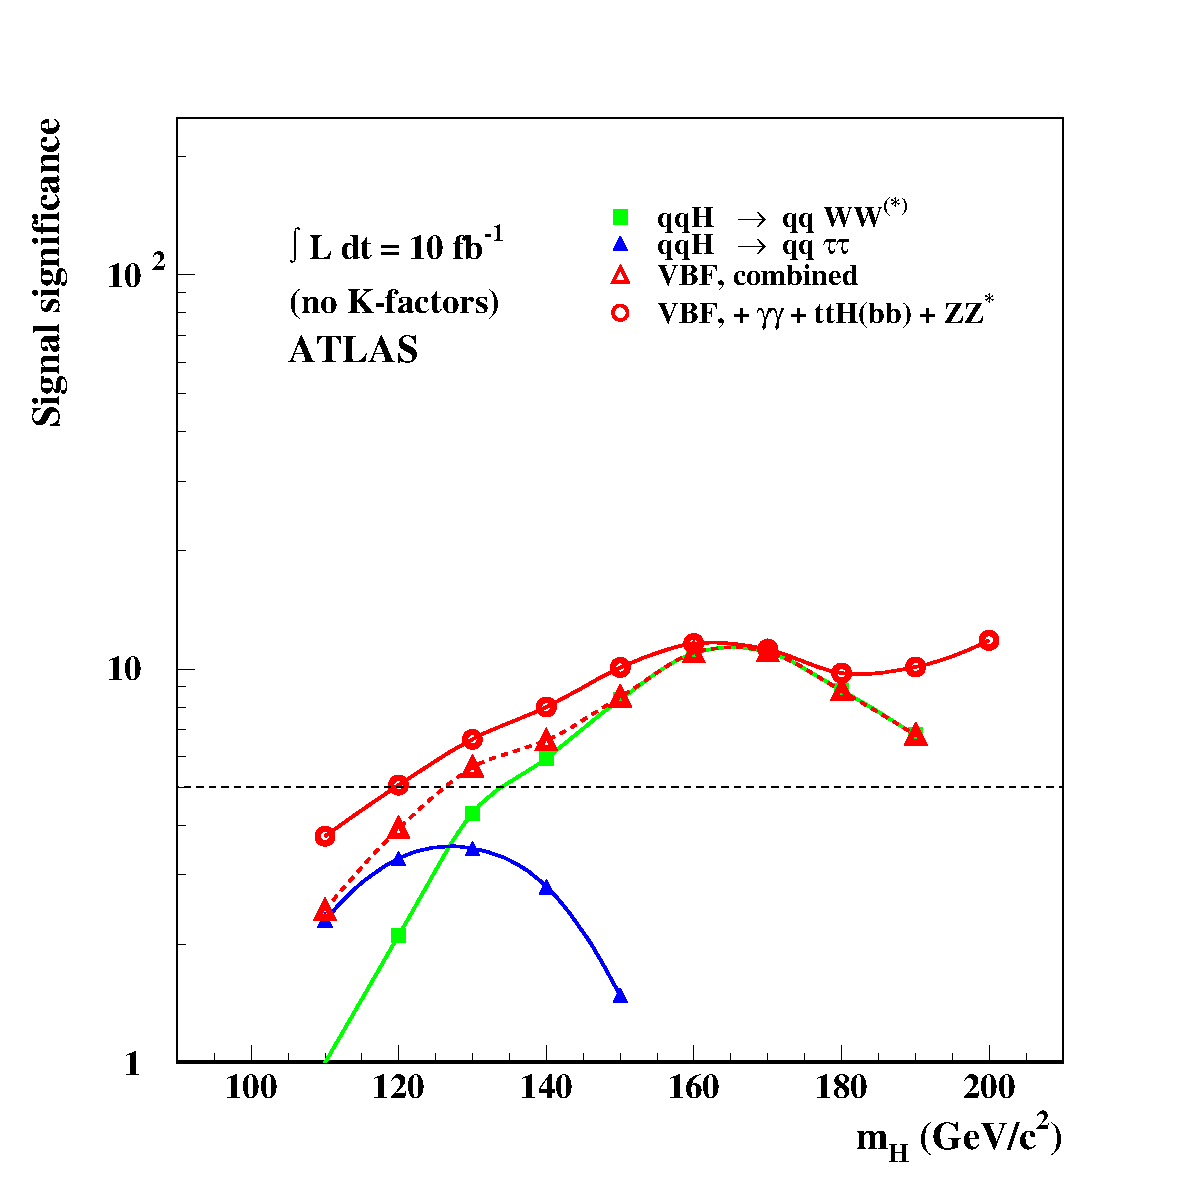
\includegraphics[width=0.6\linewidth]{graphics/vbf_sig_10fb}
	\caption{ATLAS discovery sensitivity to the Standard Model Higgs boson in the low-mass region for an integrated luminosity of 10 fb$^{-1}$. Shown are signal significances for individual channels and a combination of channels. A $\pm$10$\%$ systematic uncertainty on the background is applied to the VBF channel \cite{Buescher:2005re}.}
	\label{fig:vbfsig10fb}
\end{figure}

\section{Conclusions}
The review has summarised the theoretical foundations and experimental strategies that developed the search for the Standard Model Higgs boson, with emphasis on the dominant production modes, the key decay channels, and the experimental signatures that made discovery possible --- in particular, $H \rightarrow \gamma \gamma$ and $H \rightarrow ZZ \rightarrow 4 \ell$ --- and the role of VBF selections in improving signal-to-background ratios.\\

The Higgs production cross sections, higher-order QCD and electroweak corrections, and branching fractions were discussed. The most dominant production channel at the LHC is gluon-gluon fusion;  yet, accessing the dominant Higgs decay mode, $H \rightarrow b \bar{b}$, becomes challenging due to the indistinguishability between signal and background processes. The NLO QCD corrections increased the cross section by $\sim 50$ -- $100 \%$ and NNLO calculations gave a 10 to 20$\%$ increase above NLO. Since the gluon-gluon fusion channel produces more Higgs bosons than the other channels, it is significant in Higgs studies and improvements in higher-order calculations are essential for precision Higgs coupling analyses. Due to its topology, the vector boson fusion channel was demonstrated to be a powerful handle for suppressing backgrounds and enhancing sensitivity across several decay modes. Among VBF final states, $qqH \rightarrow WW \rightarrow \ell^+ \ell^- p_T^{\text{miss}} $  was found to be the most promising discovery channel in the 140 --190 GeV mass range due to the ability to suppress background via tagging jets associated with WW-fusion, coupled with a large signal-to-background ratio. The $qqH \rightarrow qq \tau \tau$ final state is the most promising probe of the Higgs-tau Yukawa coupling in the 110 -- 140 GeV mass range, but requires an integrated luminosity of roughly  30 fb$^{-1}$ and control of the $Z \rightarrow \tau \tau$ background. Even though the $qqH \rightarrow qq \gamma \gamma$ has a clean final state, it suffers from a small branching ratio; assuming an integrated luminosity of 30 fb$^{-1}$ yields a $2.2 \sigma$ signal significance for a $m_H = 130$ GeV Higgs.  $qqH \rightarrow qqZZ$ provides sensitivity in the heavy Higgs regime with a $3.8 \sigma$ signal significance for a $m_H = 350$ GeV Higgs, assuming an integrated luminosity of 30 fb$^{-1}$.  On the other hand, $qqH \rightarrow qq b\bar{b}$ is challenging due to a large QCD background at LO which exceeds the signal. Despite having a smaller cross-section than gluon-gluon fusion, the vector boson fusion mechanism is tree level at LO rather than loop-induced, thus, provides cleaner predictions and is a more direct probe of the weak coupling to the Higgs. In addition to gluon-gluon fusion and vector boson fusion, the Higgs-strahlung channel and associated productions with heavy quarks channel contribute to the overall search strategy. Higgs-strahlung involves the radiation of a Higgs boson off a weak gauge boson and is  valuable for low-mass Higgs searches in association with leptonic W or Z decays, which provide clean experimental signatures. Though suppressed at the LHC due to the proton-proton initial state, Higgs-strahlung --- requiring a quark-anti-quark initial state --- was significant in TeVatron's low-mass searches due to it being a proton-anti-proton collider; the quarks and anti-quarks are valence. The associated production with heavy quarks provides direct access to the Higgs-quark Yukawa couplings, especially the top–Higgs interaction. While experimentally challenging due to small cross-sections and large backgrounds, these processes are crucial in the study of fermion mass generation. These production modes complement the dominant gluon-gluon and vector-boson–fusion processes.\\

Building upon the discussion of production mechanisms, an essential aspect of understanding the Higgs boson lies in the study of its decay properties. The Higgs boson decays predominantly into the heaviest kinematically accessible fermions or bosons, with branching ratios calculated at next-to-leading order using the \verb|HDECAY| and \verb|PROPHECY4F| programmes. For Higgs masses below 140 GeV, fermionic modes, particularly $H \rightarrow b \bar{b}$ dominate, which is consistent with the mass-proportional nature of Yukawa couplings. Despite the low branching ratio --- roughly 3 orders of magnitude lower than $H \rightarrow b\bar{b}$ --- the $H \rightarrow \gamma \gamma$ channel provides clean signatures that led to an accurate reconstruction of the invariant-mass and was crucial to the discovery. At mass regions above 180 GeV, both W and Z boson pairs become on-shell and the Higgs decay via vector bosons become increasingly significant. Out of all possible decay routes, the $ZZ \rightarrow 4\ell$ provided a cleaner final state, excellent mass resolution and thus is a discovery channel for the Higgs Boson.\\

 A combination of theoretical efforts, advanced analysis techniques, high-resolution channels and high-yield modes enabled the discovery of the Higgs boson at the LHC. Looking forward, upgrades in luminosity and analysis techniques, including improved jet and lepton identification, will lead to a reduction in statistical and systematic uncertainties. This makes measurements more precise, thus enables one to exclude or better quantify possible deviations from the Standard Model. Improved theoretical predictions, including higher-order QCD and electroweak corrections and improved parton distribution functions, will reduce theory uncertainties. In parallel, searches for additional Higgs bosons and signatures of extended Higgs sectors, such as those predicted in two-Higgs doublet models, supersymmetry, and other beyond the Standard Model frameworks, will test the completeness of the Higgs sector. In summary, the combined theoretical and experimental efforts described here not only enabled the Higgs discovery but also established a robust framework for precision Higgs physics experiments that will follow.




\bibliographystyle{JHEP}
\bibliography{refs}

\end{document}
